\documentclass[12pt]{article}
\usepackage[a4paper, margin=1in]{geometry}
\usepackage{enumitem}
\usepackage{titlesec}
\usepackage{graphicx}
\usepackage{hyperref}
\usepackage{float}
\titleformat{\section}{\Large\bfseries}{\thesection}{1em}{}
\titleformat{\subsection}{\large\bfseries}{\thesubsection}{1em}{}
\title{User Manual\\Taxi Tap by Git It Done}
\date{}
\begin{document}
\maketitle
\begin{figure}[H]
  \centering
  
\includegraphics[width=0.5\textwidth]{LogoGroup.png} 
\end{figure}
\begin{figure}[H]
  \centering
  
\includegraphics[width=0.5\textwidth]{LogoTaxiTap.png} 
\end{figure}
\newpage
\tableofcontents
\newpage

\section{Getting Started}

\subsection{Landing Page}

When you first open the TaxiTap app, you'll be greeted by the Landing Page which provides:

\subsubsection{App Overview}
The landing page displays a brief overview of TaxiTap's key features:
\begin{itemize}
    \item Quick and reliable taxi booking
    \item Real-time tracking and navigation
    \item Driver and passenger safety features
    \item Multi-language support
\end{itemize}

\subsubsection{Language Selection}
TaxiTap supports multiple South African languages to ensure accessibility for all users:
\begin{itemize}
    \item English (Default)
    \item isiZulu
    \item Setswana
    \item Afrikaans
\end{itemize}

You can change the app language at any time by selecting your preferred language from the language selector on the landing page. This will translate the entire app interface into your chosen language.

\begin{figure}[H]
  \centering
  \includegraphics[width=0.4\textwidth]{landing_page.png}
  \caption{Landing Page with App Overview}
\end{figure}

\begin{figure}[H]
  \centering
  \includegraphics[width=0.4\textwidth]{language_selection.png}
  \caption{Language Selection Options}
\end{figure}

\begin{figure}[H]
  \centering
  \includegraphics[width=0.4\textwidth]{ttap_tn.png}
  \caption{TaxiTap in Setswana}
\end{figure}

From the landing page, you can proceed to either sign up for a new account or log in to your existing account.

\subsection{Logging In and Signing Up}

TaxiTap provides separate interfaces for passengers and drivers. To get started, you'll need to create an account or log in to your existing account.

\subsubsection{Sign Up}
To create a new account, you'll need to provide the following information:
\begin{itemize}
    \item Full Name
    \item Phone Number
    \item Password
    \item Role (Passenger or Driver)
\end{itemize}

\begin{figure}[H]
  \centering
  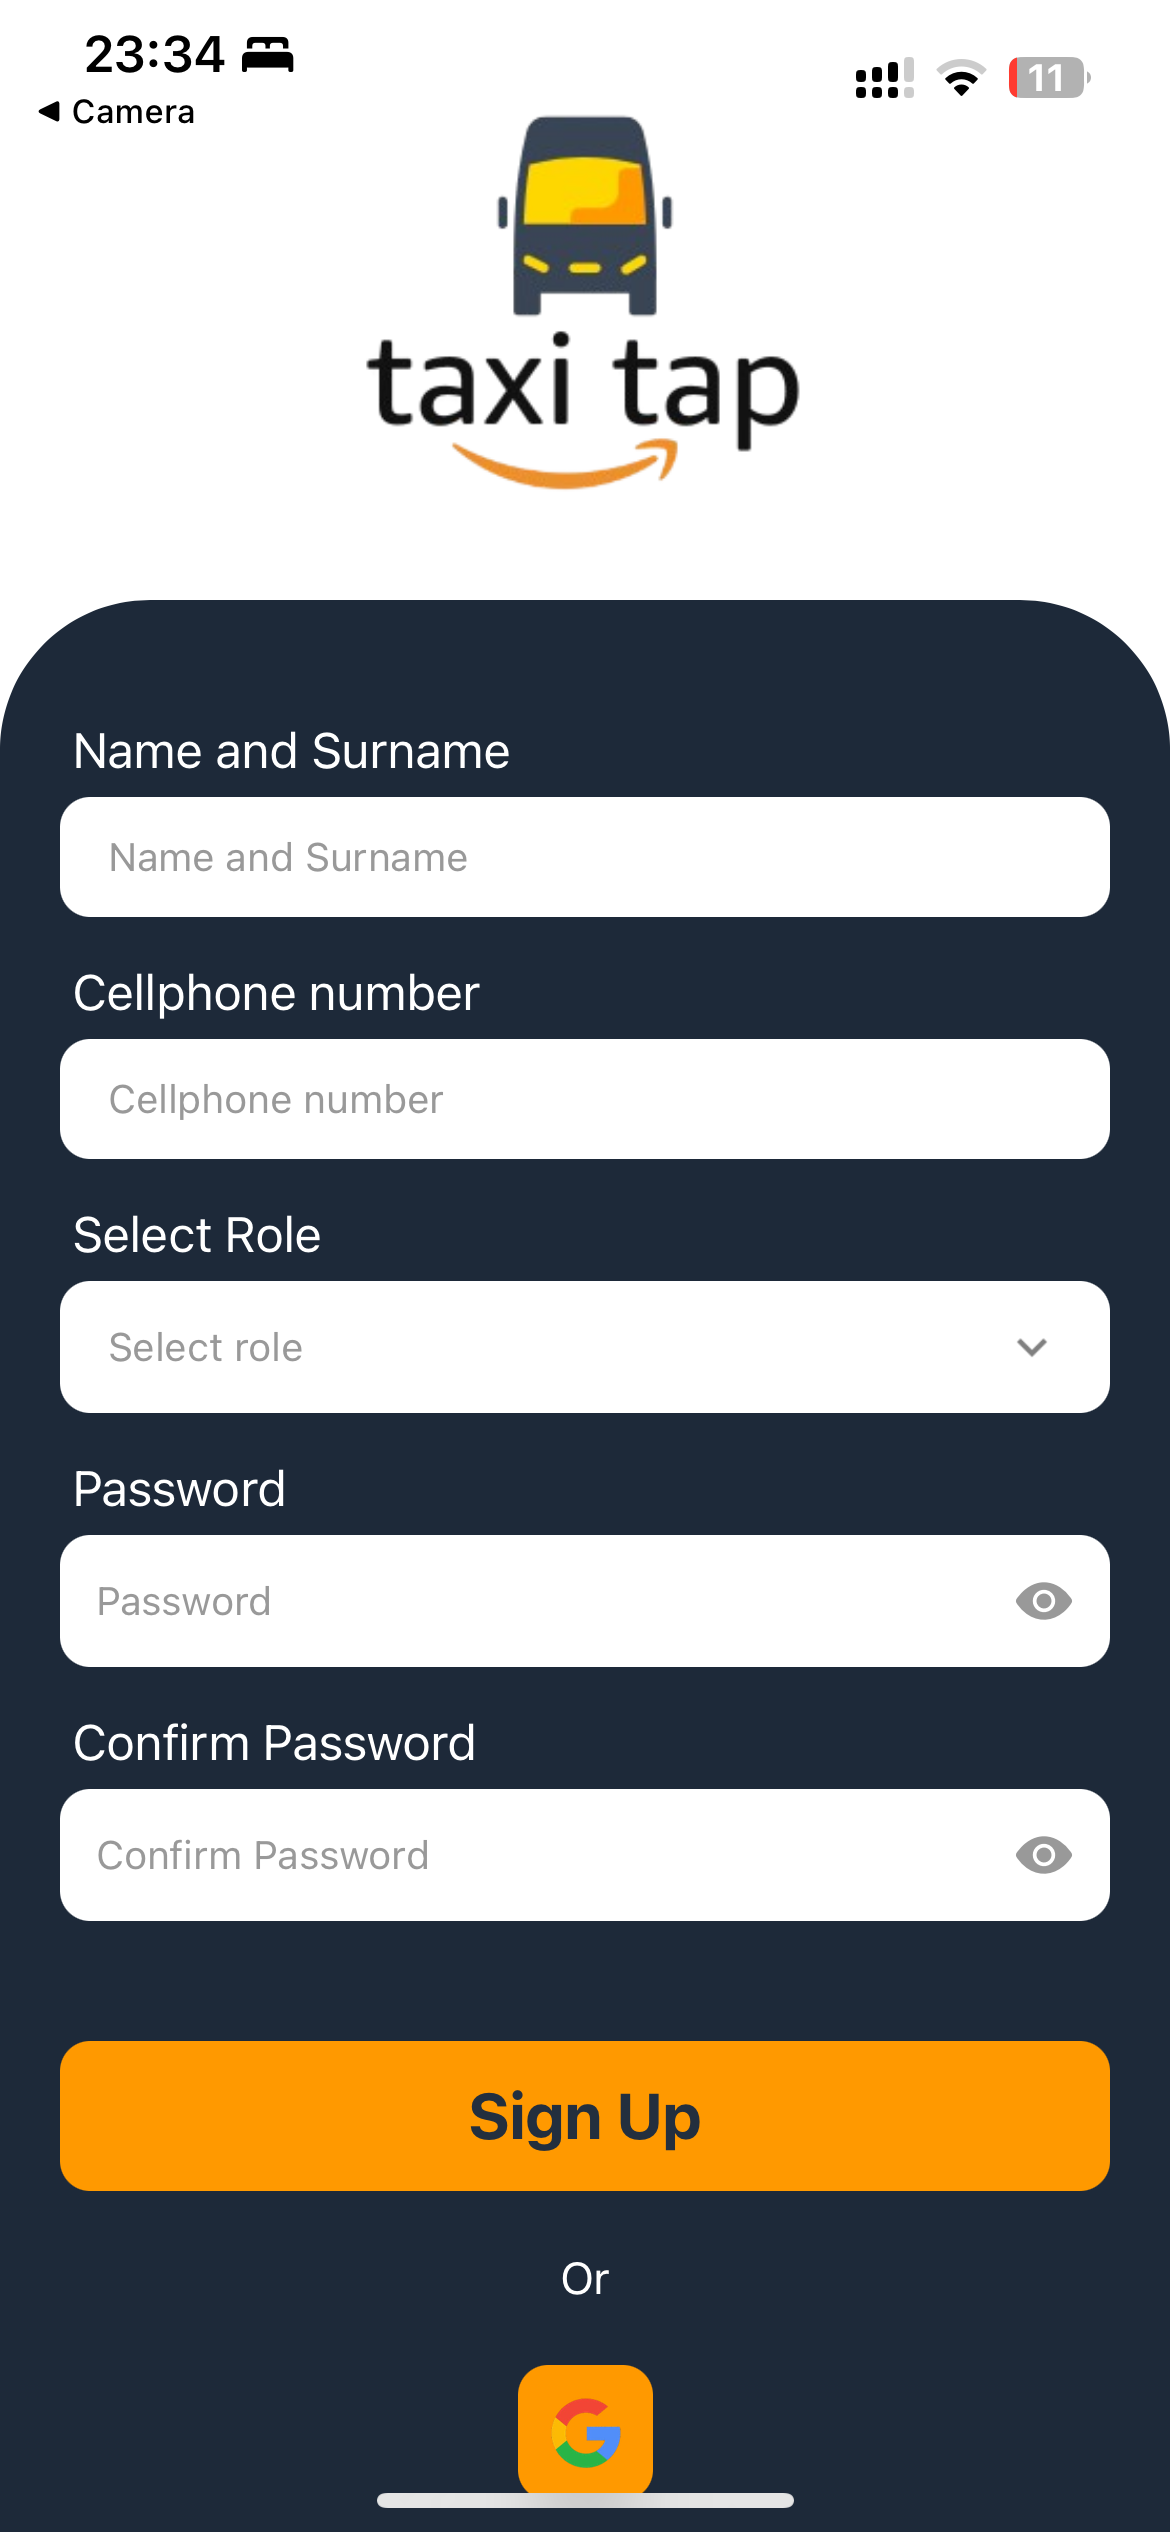
\includegraphics[width=0.4\textwidth]{signup2.png}
  \caption{Sign Up Screen}
\end{figure}

\begin{figure}[H]
  \centering
  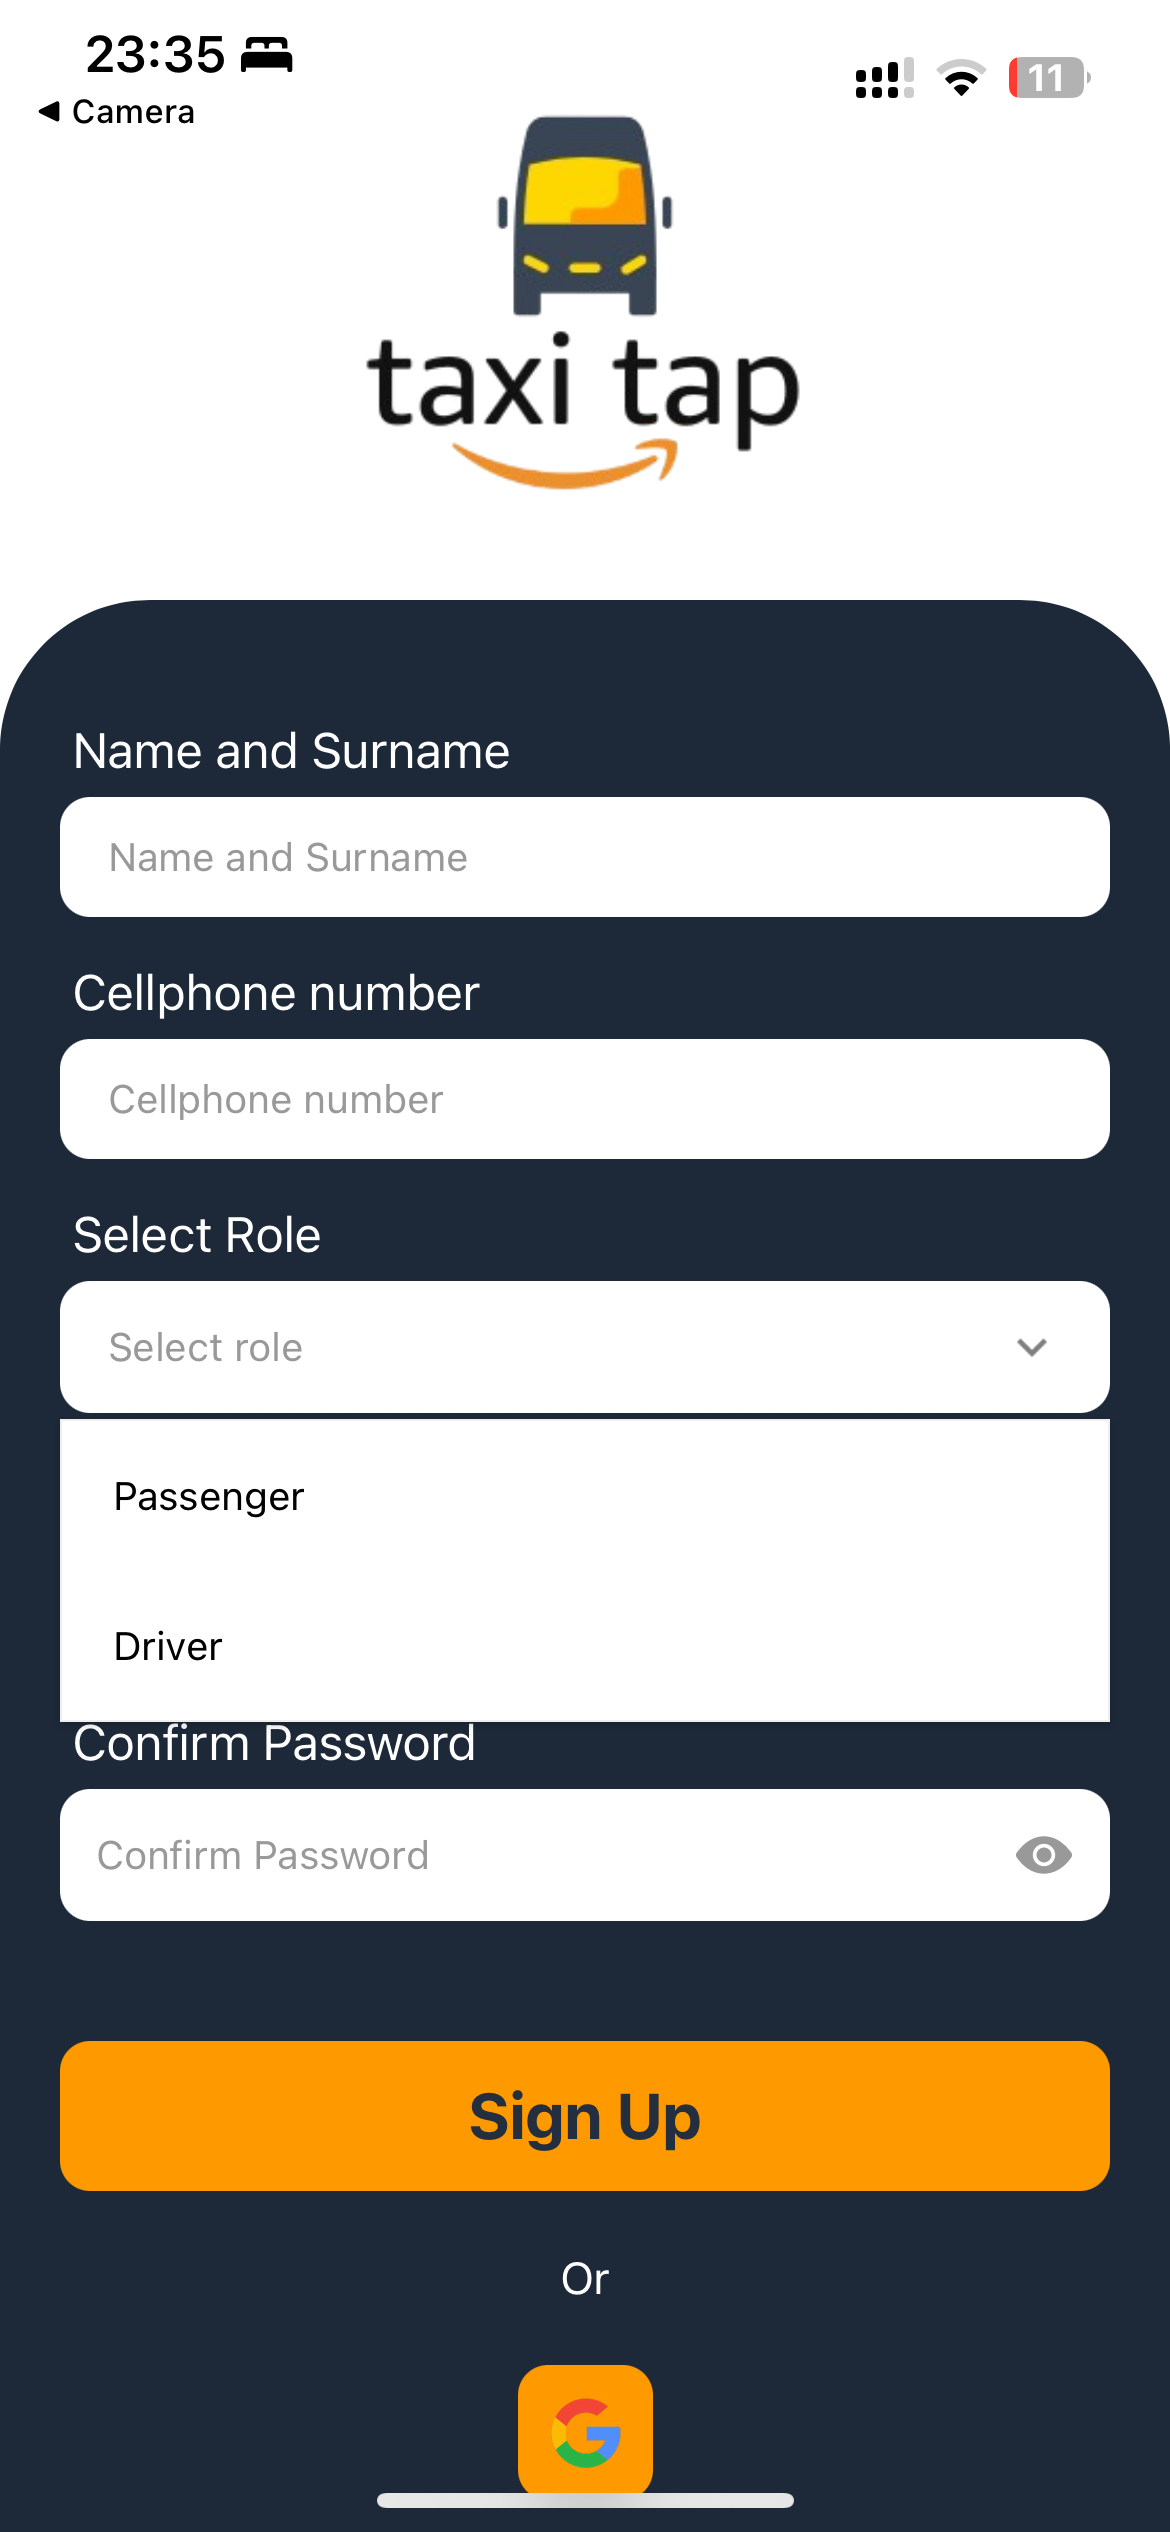
\includegraphics[width=0.4\textwidth]{signup_roles.png}
  \caption{Sign Up Screen}
\end{figure}

\subsubsection{Log In}
To log in to your existing account, you'll need:
\begin{itemize}
    \item Phone Number
    \item Password
\end{itemize}

\begin{figure}[H]
  \centering
  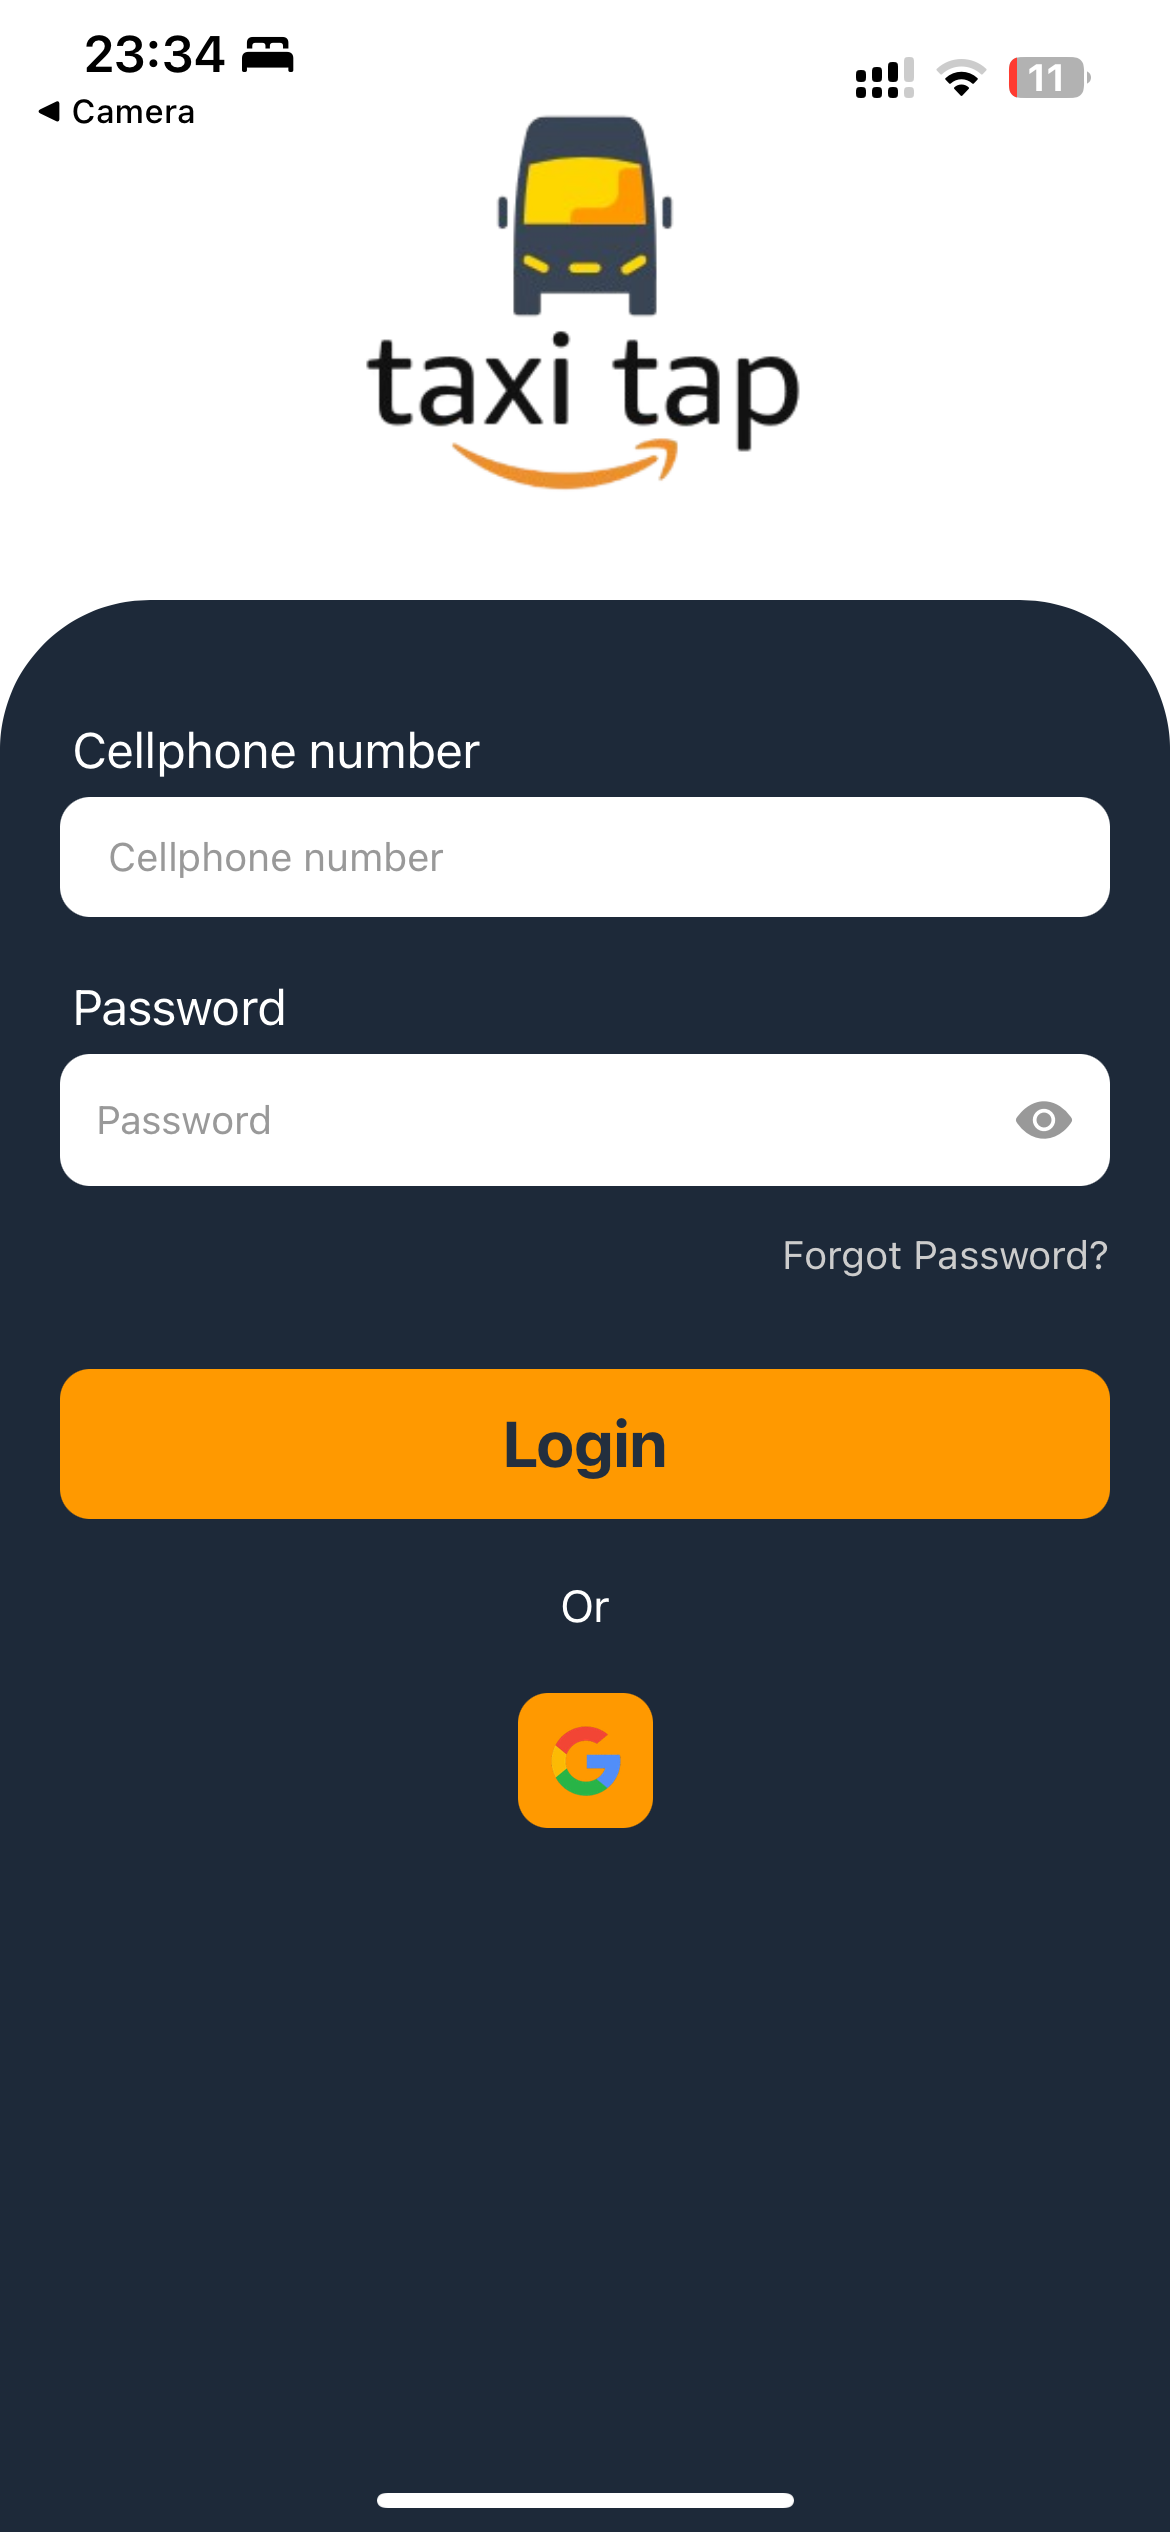
\includegraphics[width=0.6\textwidth]{login2.png}
  \caption{Login Screen}
\end{figure}

\newpage

\section{Passenger Interface}

\subsection{Requesting a Ride}

\subsubsection{Step 1: Enter Destination Details}
\begin{enumerate}
    \item Open the TaxiTap app and ensure you're logged in as a passenger
    \item On the main screen, you'll see a map with your current location
    \item Type in your destination address in the destination field
    \item The system will automatically detect your current location as the origin, or you can manually enter your pickup address
\end{enumerate}

\begin{figure}[H]
  \centering
  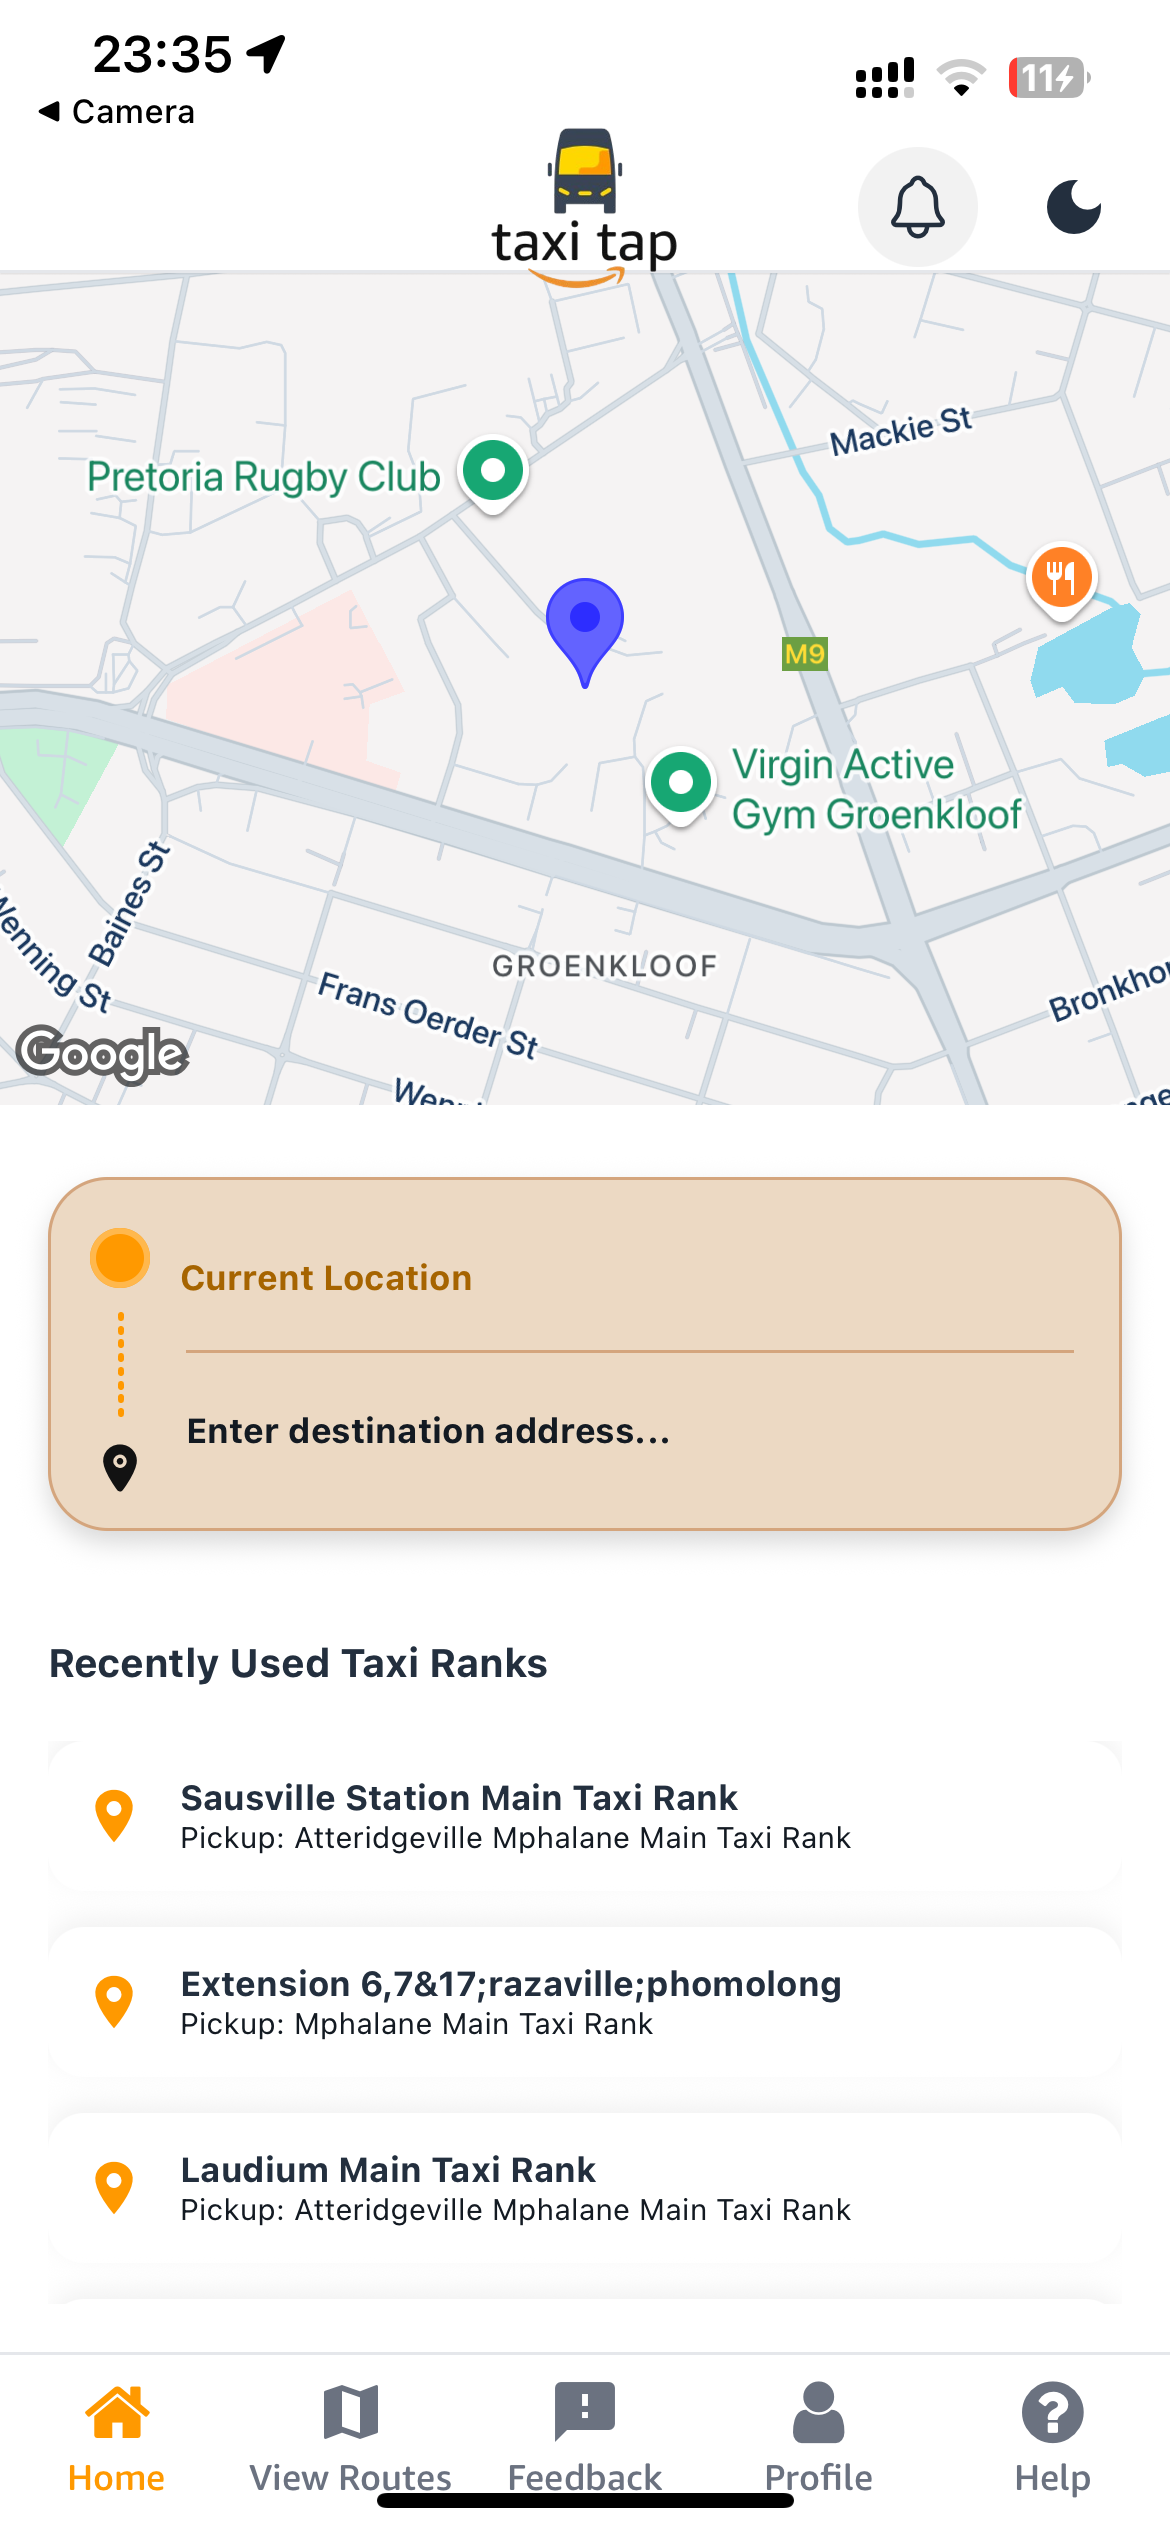
\includegraphics[width=0.4\textwidth]{destination_entry.png}
  \caption{Entering Destination}
\end{figure}

\subsubsection{Step 2: Check for Available Taxis}
The app will search for available taxis that:
\begin{itemize}
    \item Are nearby your location
    \item Follow routes with stops near both your origin and destination
\end{itemize}

If taxis are available, you'll see:
\begin{itemize}
    \item An orange "Reserve a Seat" button with the number of taxis available to accommodate your request.
\end{itemize}

\subsubsection{Step 3: Reserve Your Seat}
Once available taxis are found, click the orange "Reserve a Seat" button to proceed to taxi selection.

\subsection{Selecting Your Driver and Taxi}

\subsubsection{Available Taxis Page}
After clicking "Reserve a Seat," you'll be taken to the "Available Taxis" page where you can see:

\begin{itemize}
    \item Driver name and details
    \item Vehicle information (make, model, license plate)
    \item Route information
    \item Estimated fare
    \item Estimated duration
    \item Driver's current distance from you
    \item Driver rating (5-star system)
\end{itemize}

\begin{figure}[H]
  \centering
  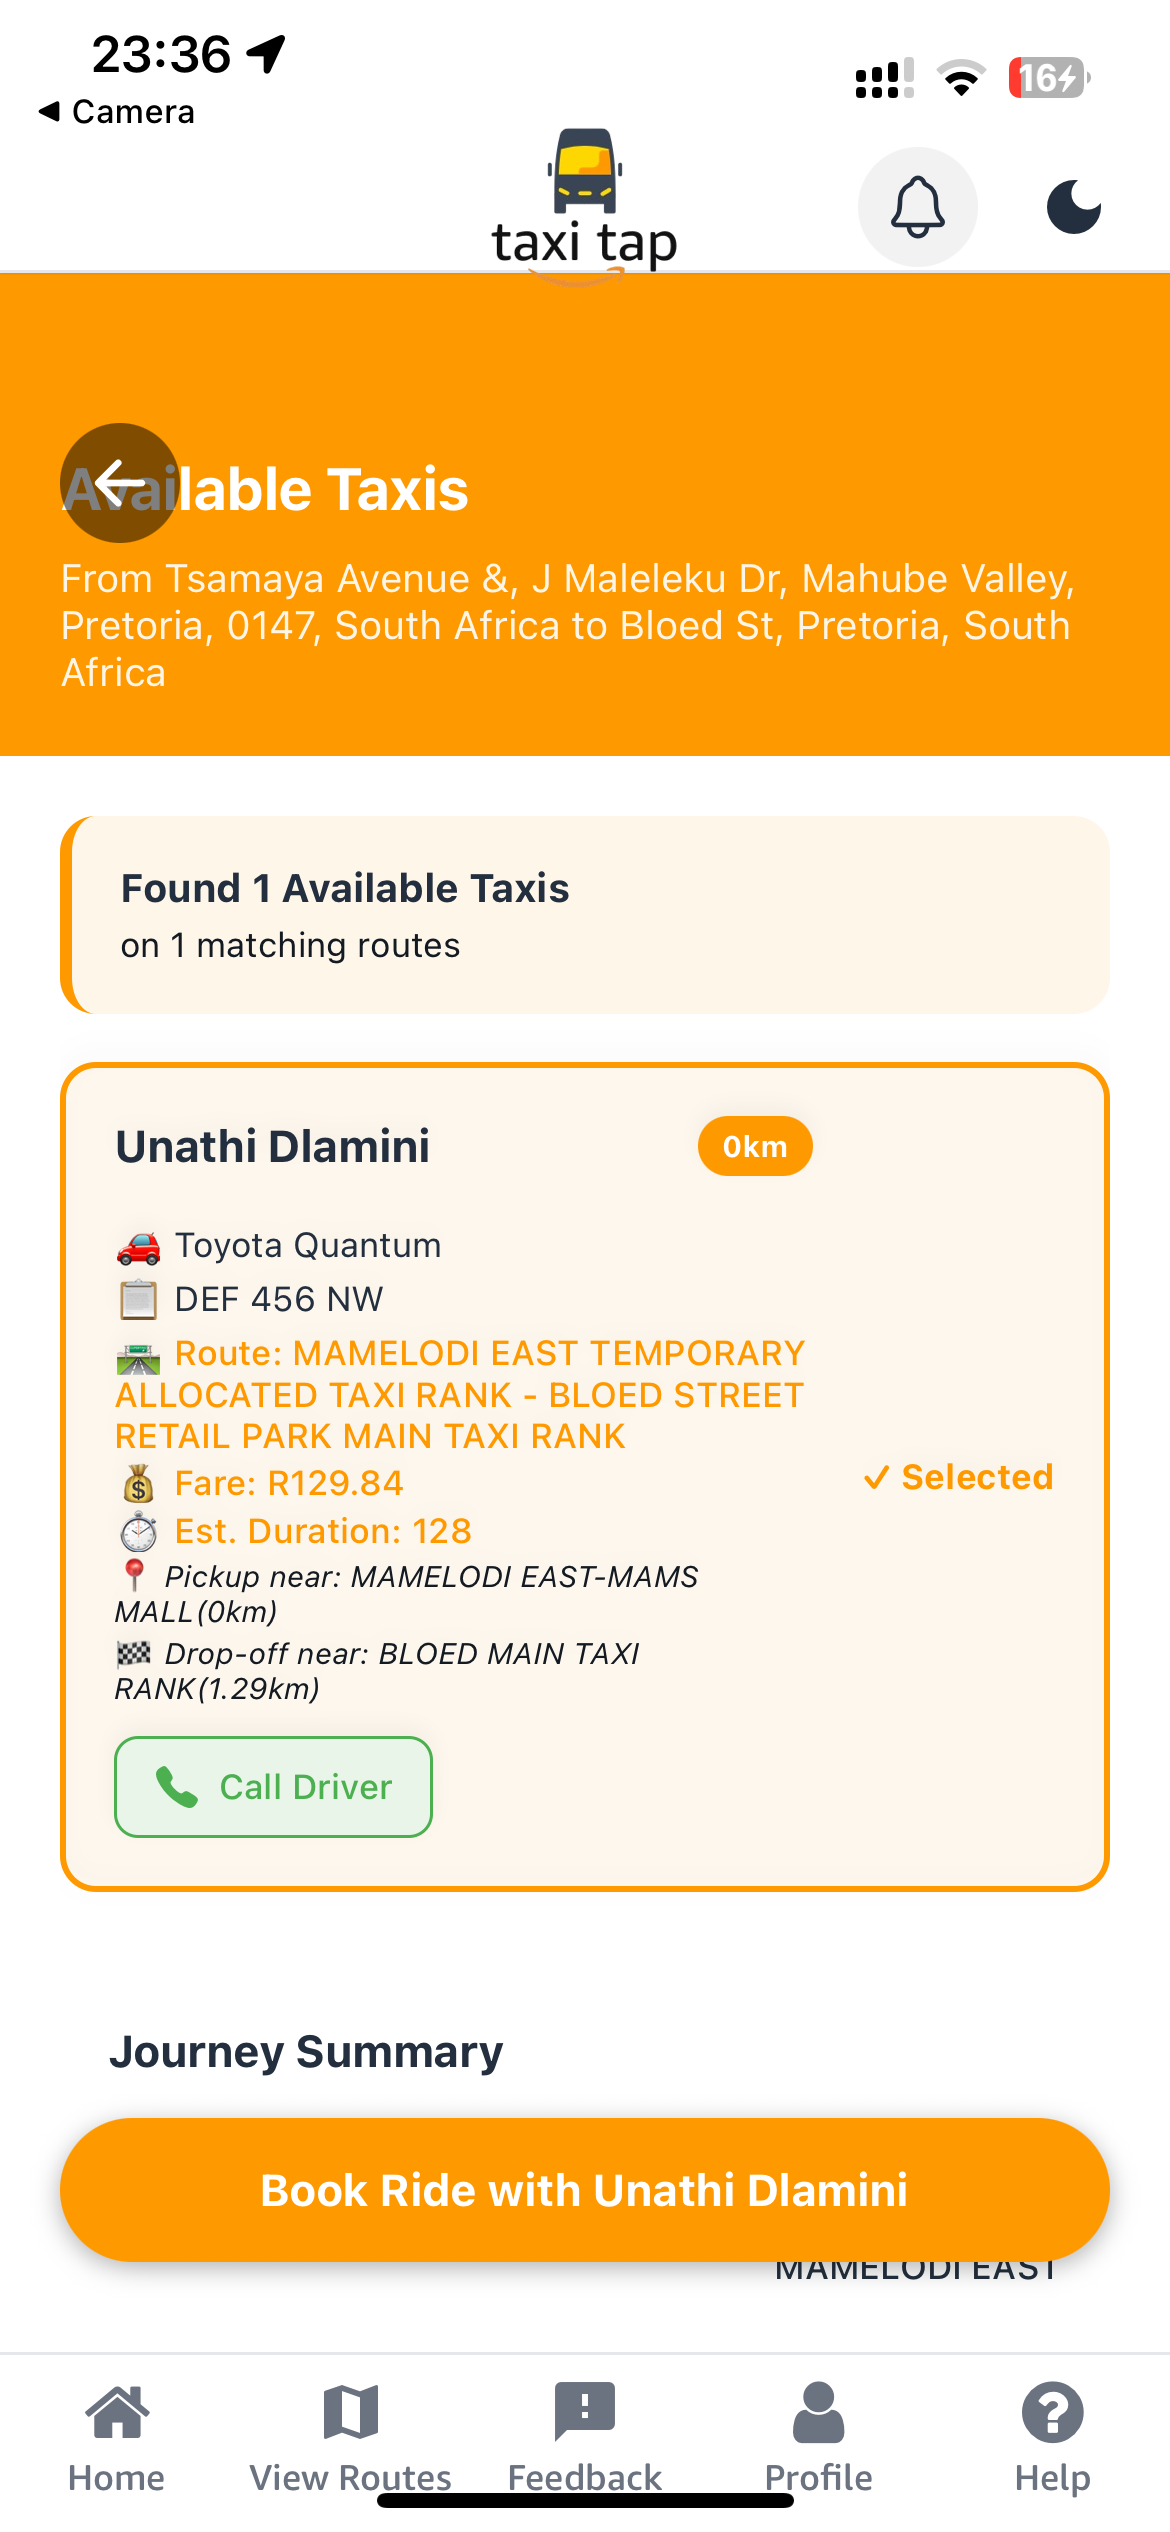
\includegraphics[width=0.4\textwidth]{taxi_selection.png}
  \caption{Taxi Selection Screen}
\end{figure}

\subsubsection{Step 4: Book Your Ride}
\begin{enumerate}
    \item Review the taxi and driver information
    \item Check the fare and estimated duration
    \item Click the orange "Book Ride with [Driver's Name]" button
    \item You can also use the "Call Driver" button to contact the driver directly
\end{enumerate}

\subsection{Managing Your Ride Request}

\subsubsection{Ride Request Sent}
After booking, you'll see a confirmation that your ride request has been sent to the driver. At this stage:
\begin{itemize}
    \item The driver will be notified of your request
    \item You'll receive a notification when the driver responds
    \item You can still cancel the request if needed
\end{itemize}

\begin{figure}[H]
  \centering
  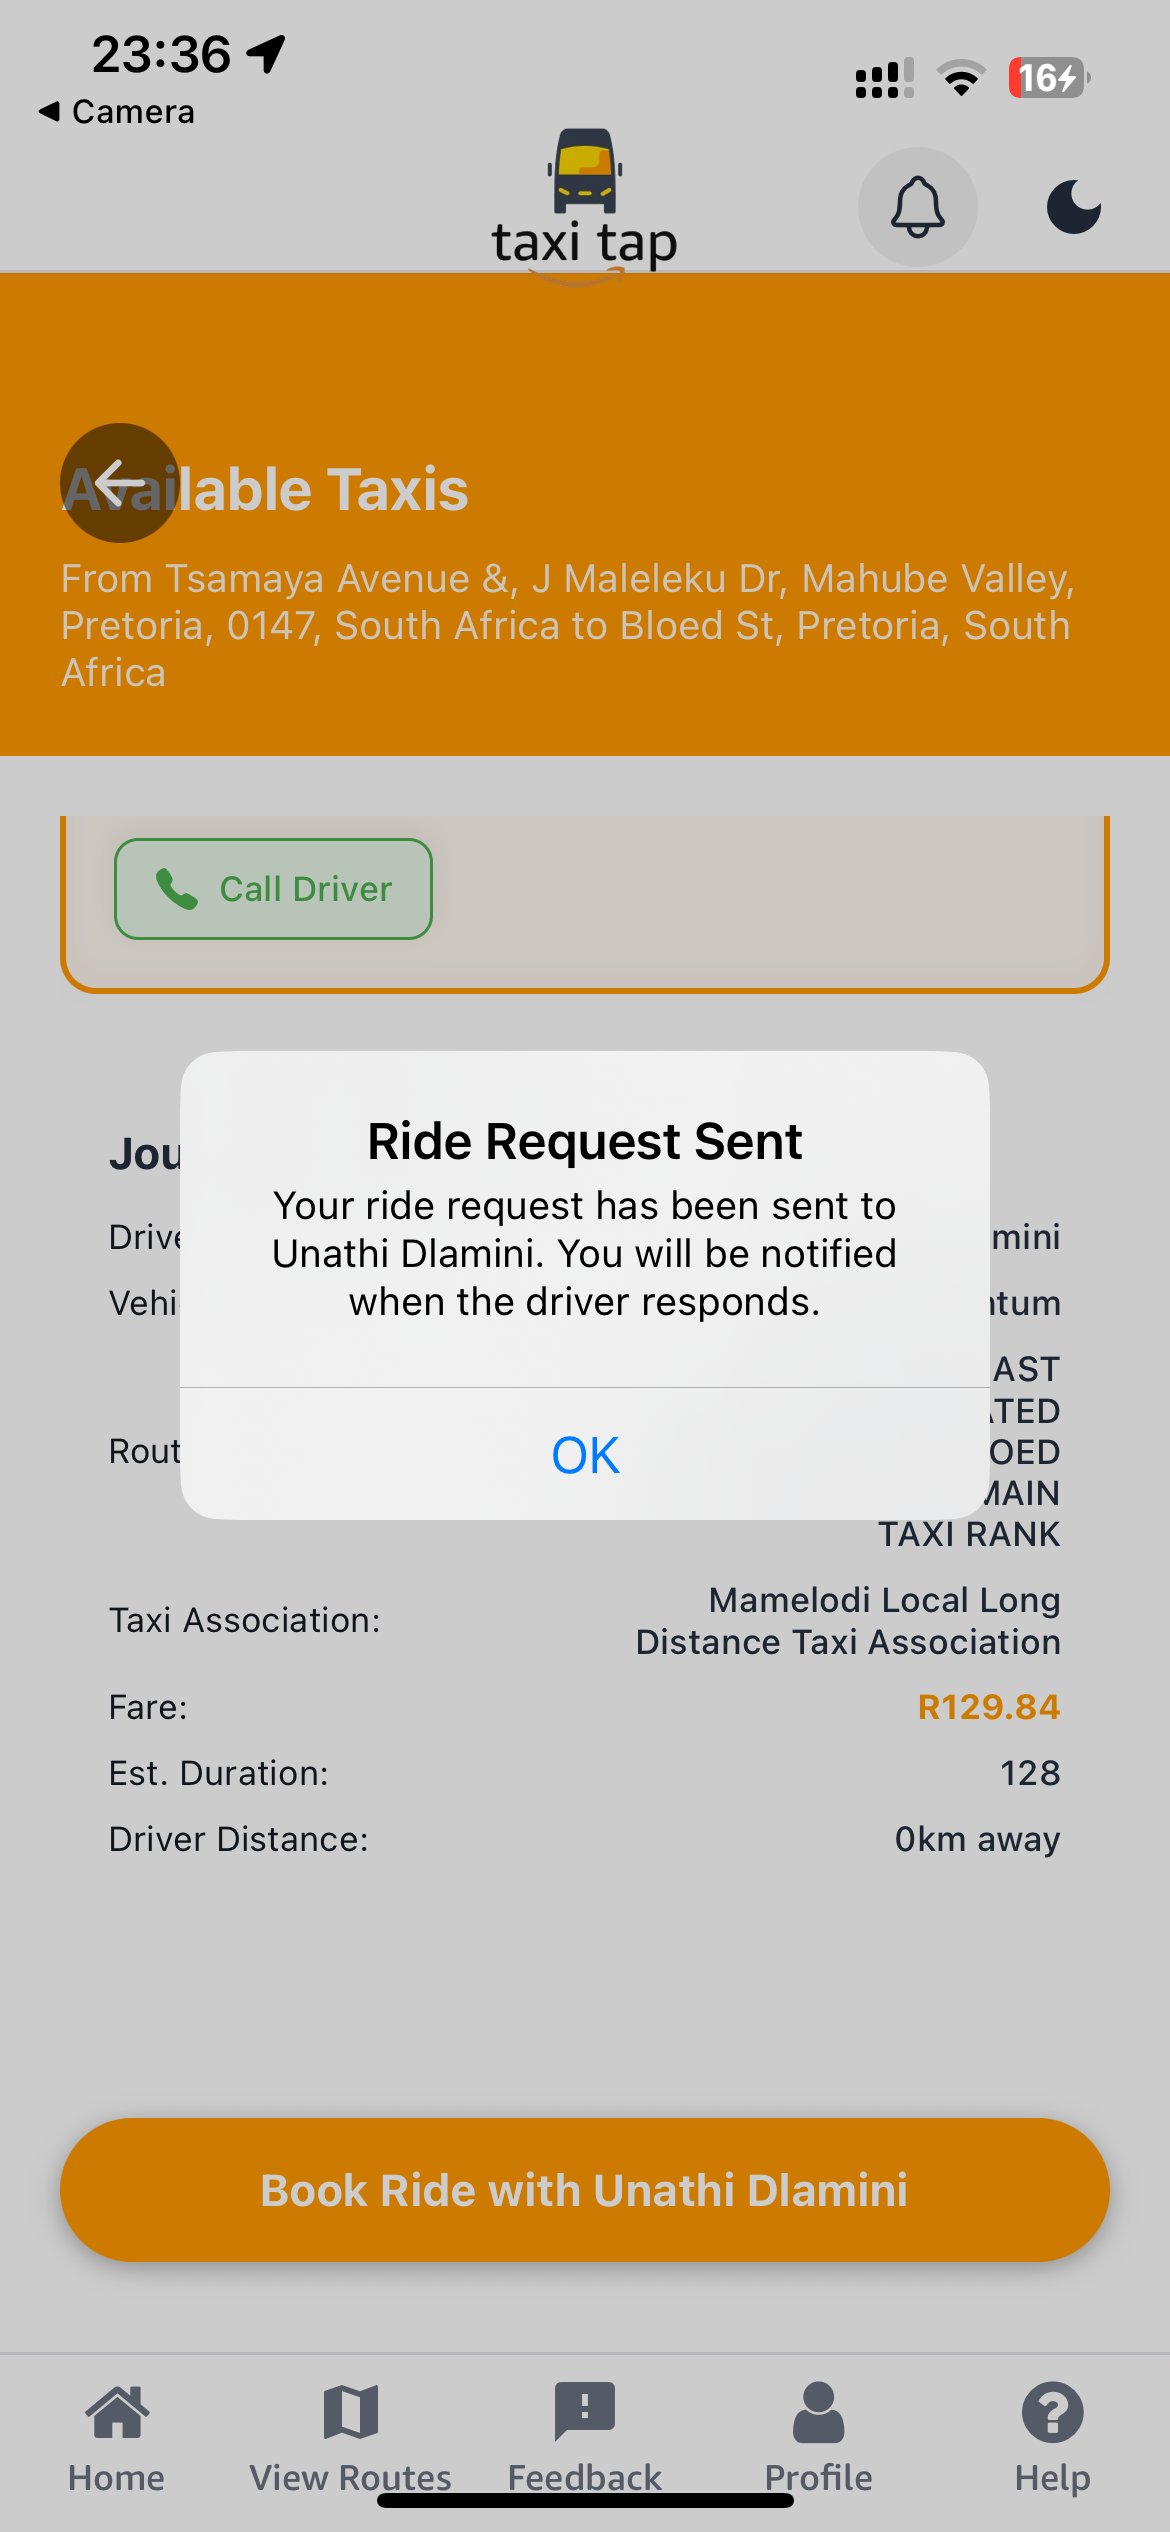
\includegraphics[width=0.4\textwidth]{ride_request_sent.png}
  \caption{Ride Request Sent Confirmation}
\end{figure}

\subsubsection{Ride Accepted}
When the driver accepts your request:
\begin{itemize}
    \item You'll receive a "Ride Accepted" notification
    \item The message will confirm "Your ride has been accepted. Driver is on the way!"
    \item You can track the driver's location on the map
    \item The "Start Ride" button will become available
\end{itemize}

\begin{figure}[H]
  \centering
  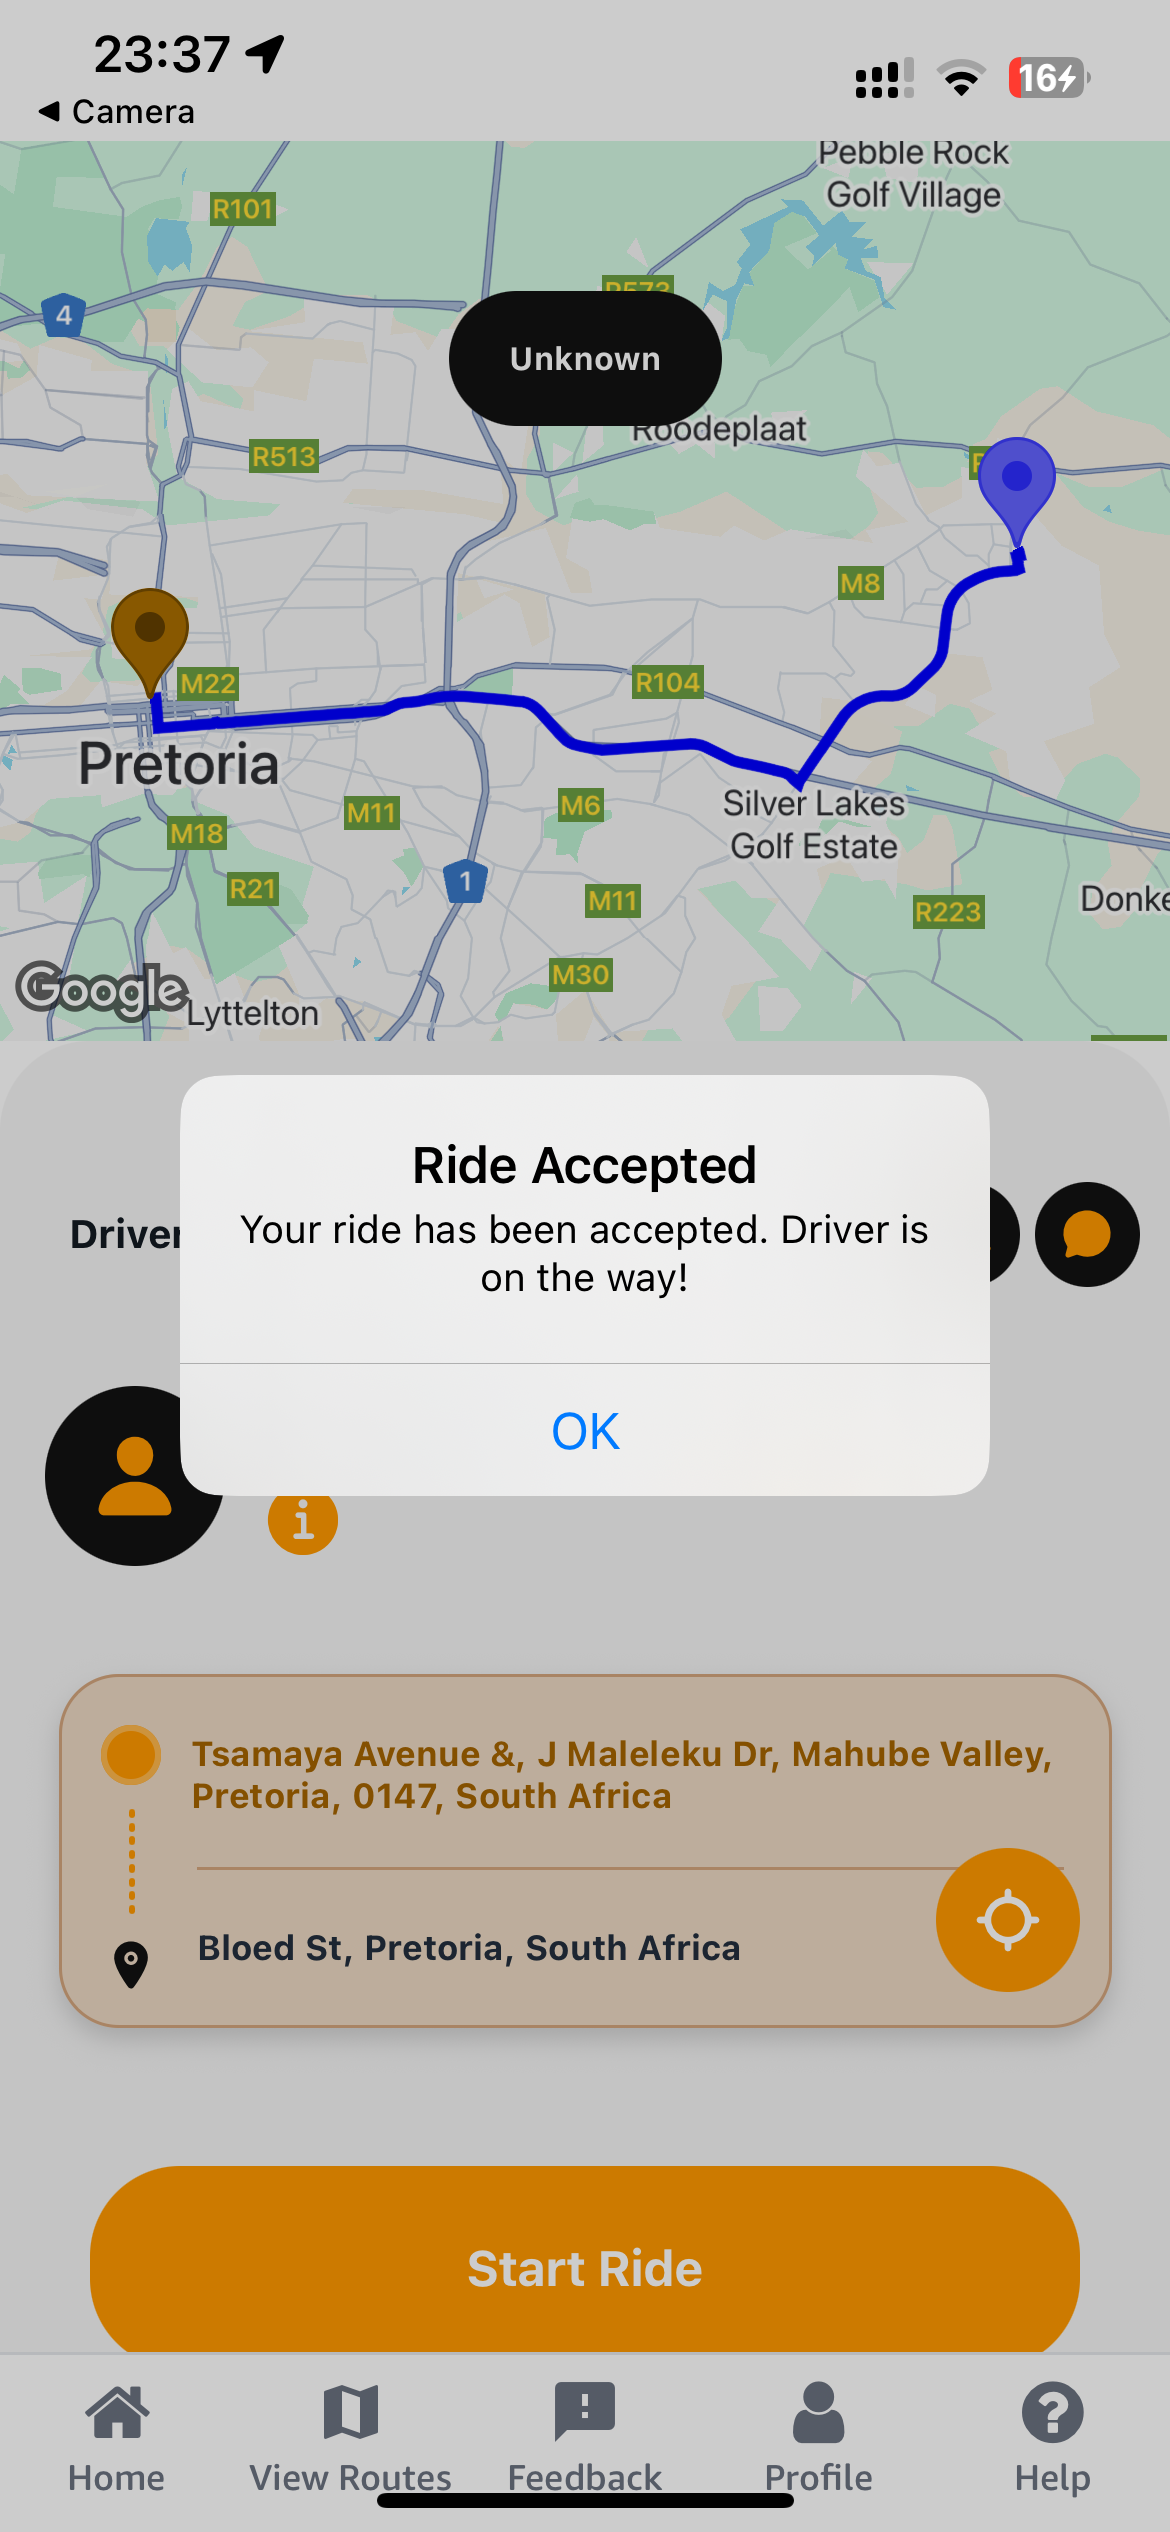
\includegraphics[width=0.4\textwidth]{ride_accepted.png}
  \caption{Ride Accepted Notification}
\end{figure}

\subsection{Starting and Managing Your Ride}

\subsubsection{Verify PIN}
When you're ready to start your ride:
\begin{enumerate}
    \item Click "Verify PIN"
    \item You'll be taken to a PIN verification page where you enter the correct PIN provided by the driver
    \item This ensures secure boarding and prevents unauthorized ride starts
\end{enumerate}

\begin{figure}[H]
  \centering
  \includegraphics[width=0.4\textwidth]{verify_pin.png}
  \caption{PIN Verification Screen}
\end{figure}

\subsubsection{Payment Confirmation}
After entering the correct PIN:
\begin{enumerate}
    \item You'll be directed to a payment confirmation page
    \item Choose whether you have paid or not
    \item This helps track payment status for both you and the driver
\end{enumerate}

\begin{figure}[H]
  \centering
  \includegraphics[width=0.4\textwidth]{payment_confirmation.png}
  \caption{Payment Confirmation Screen}
\end{figure}

\subsubsection{During the Ride}
After payment confirmation, you'll see your ride page which displays:
\begin{itemize}
    \item Your route to the destination on the map
    \item Driver details and rating
    \item Real-time journey progress
    \item Emergency contact options if needed
\end{itemize}

\begin{figure}[H]
  \centering
  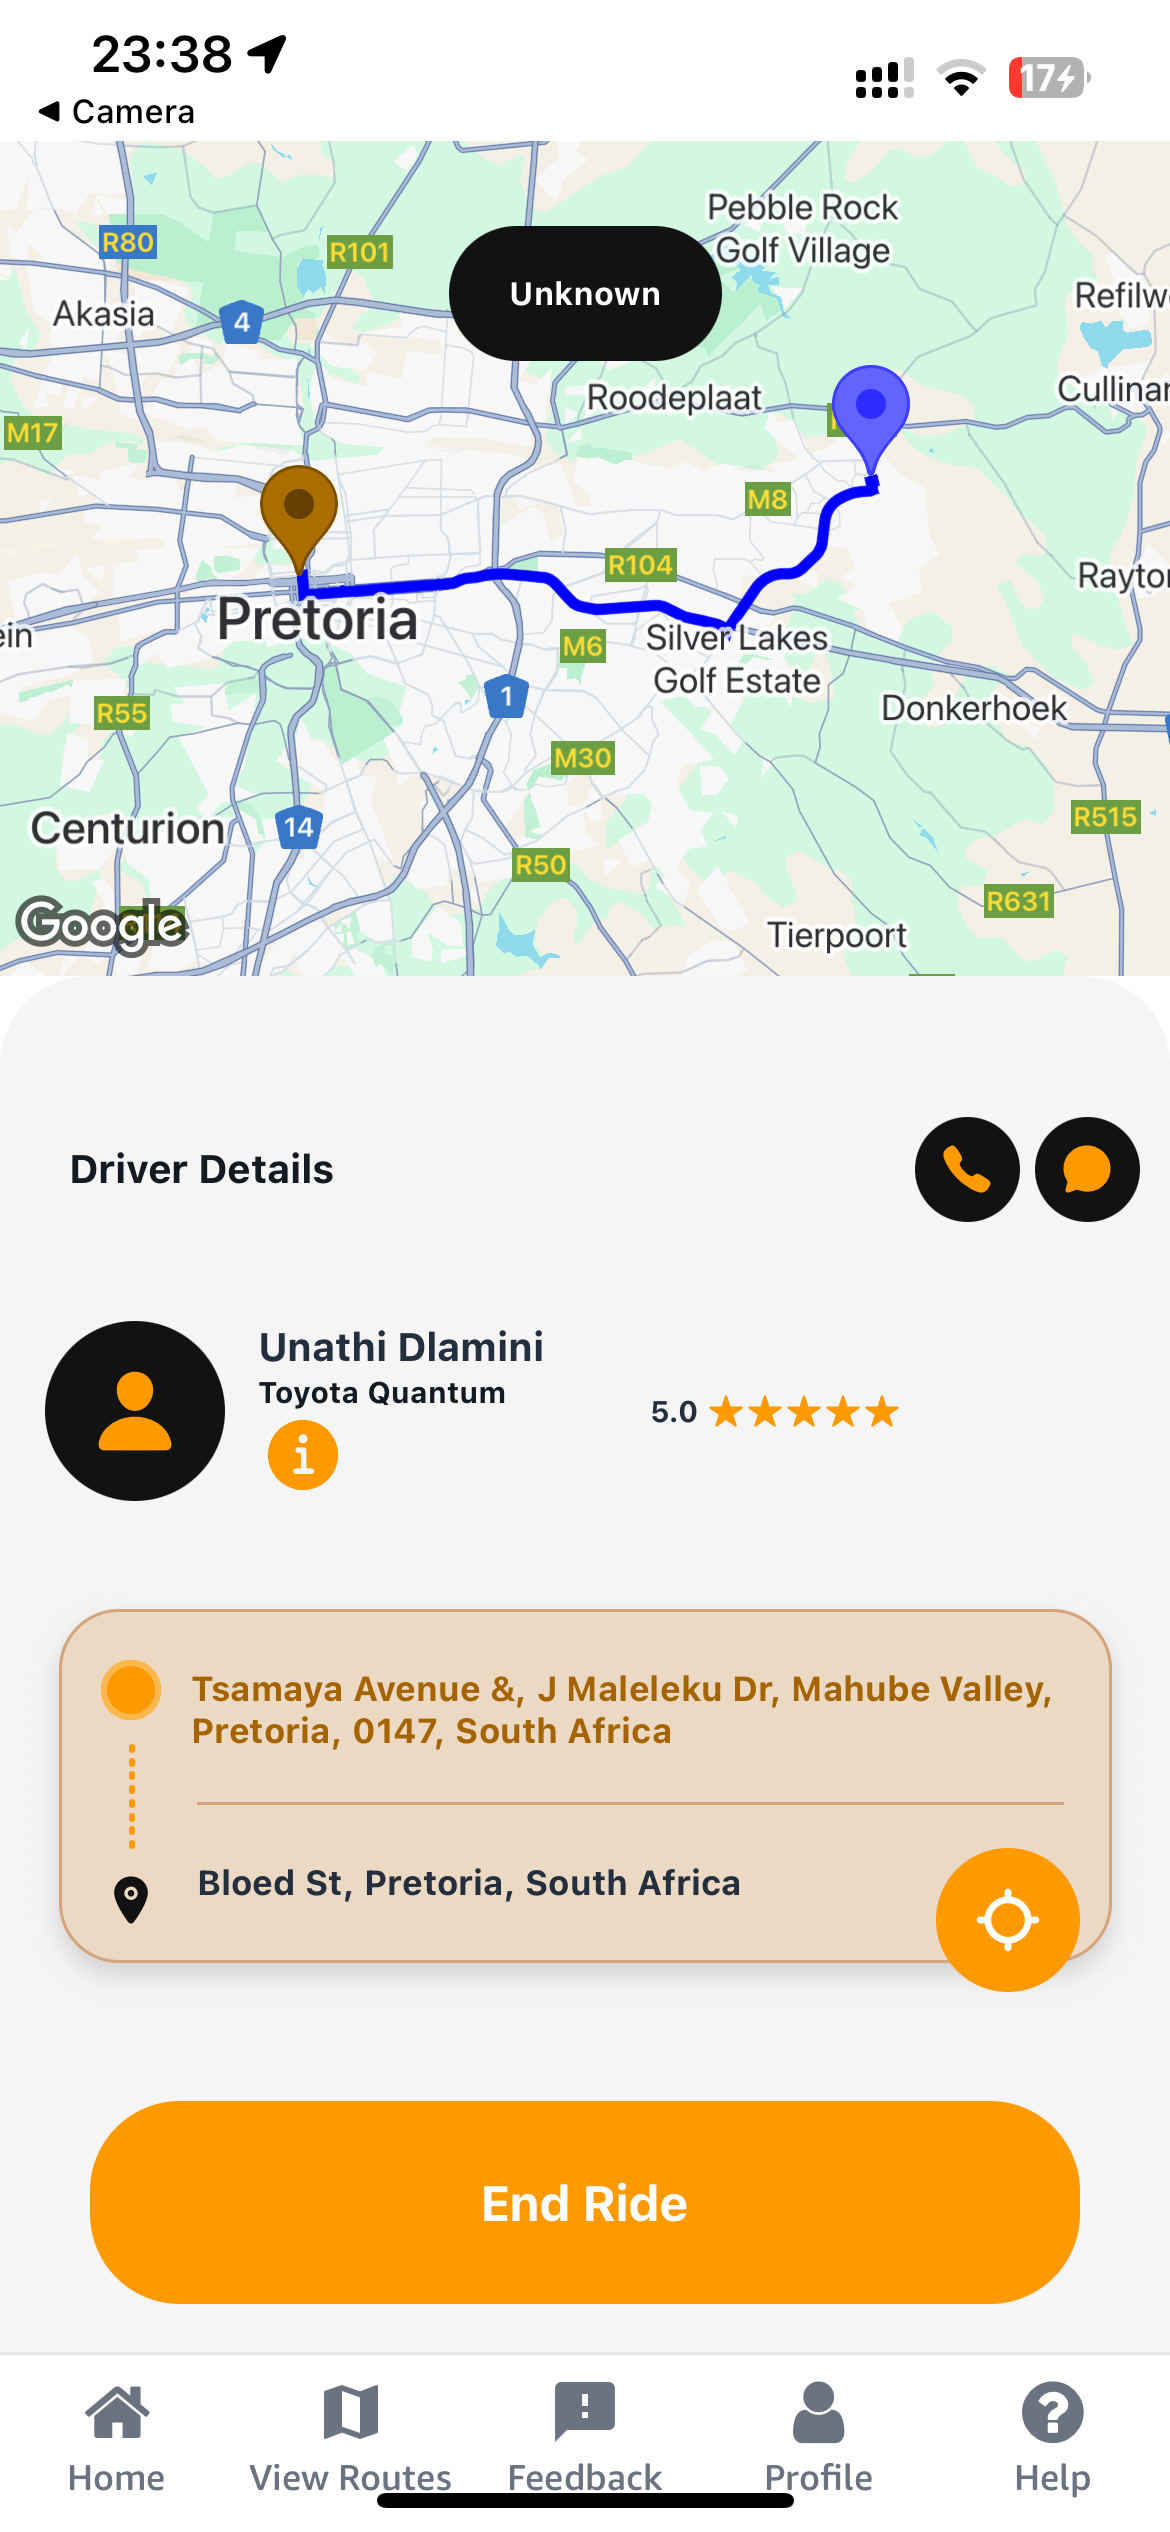
\includegraphics[width=0.4\textwidth]{during_ride.png}
  \caption{During Ride Interface}
\end{figure}

\subsubsection{Ending Your Ride}
When you reach your destination:
\begin{enumerate}
    \item Click the "End Ride" button
    \item If you have paid: You'll be directed to the Feedback page
    \item If you haven't paid: You'll be taken to the Payments page first, then to Feedback
\end{enumerate}

\begin{figure}[H]
  \centering
  \includegraphics[width=0.4\textwidth]{feedback_1.png}
  \caption{Feedback Page }
\end{figure}

\begin{figure}[H]
  \centering
  \includegraphics[width=0.4\textwidth]{feedback_page.png}
  \caption{Feedback Page}
\end{figure}

\subsection{Cancelling a Ride}

You can cancel your ride request at any time before the driver accepts it:
\begin{itemize}
    \item Click "Cancel Request" on the ride tracking screen
    \item You'll receive a "Success - Ride cancelled" confirmation
    \item The app will return to the main screen
\end{itemize}

\begin{figure}[H]
  \centering
  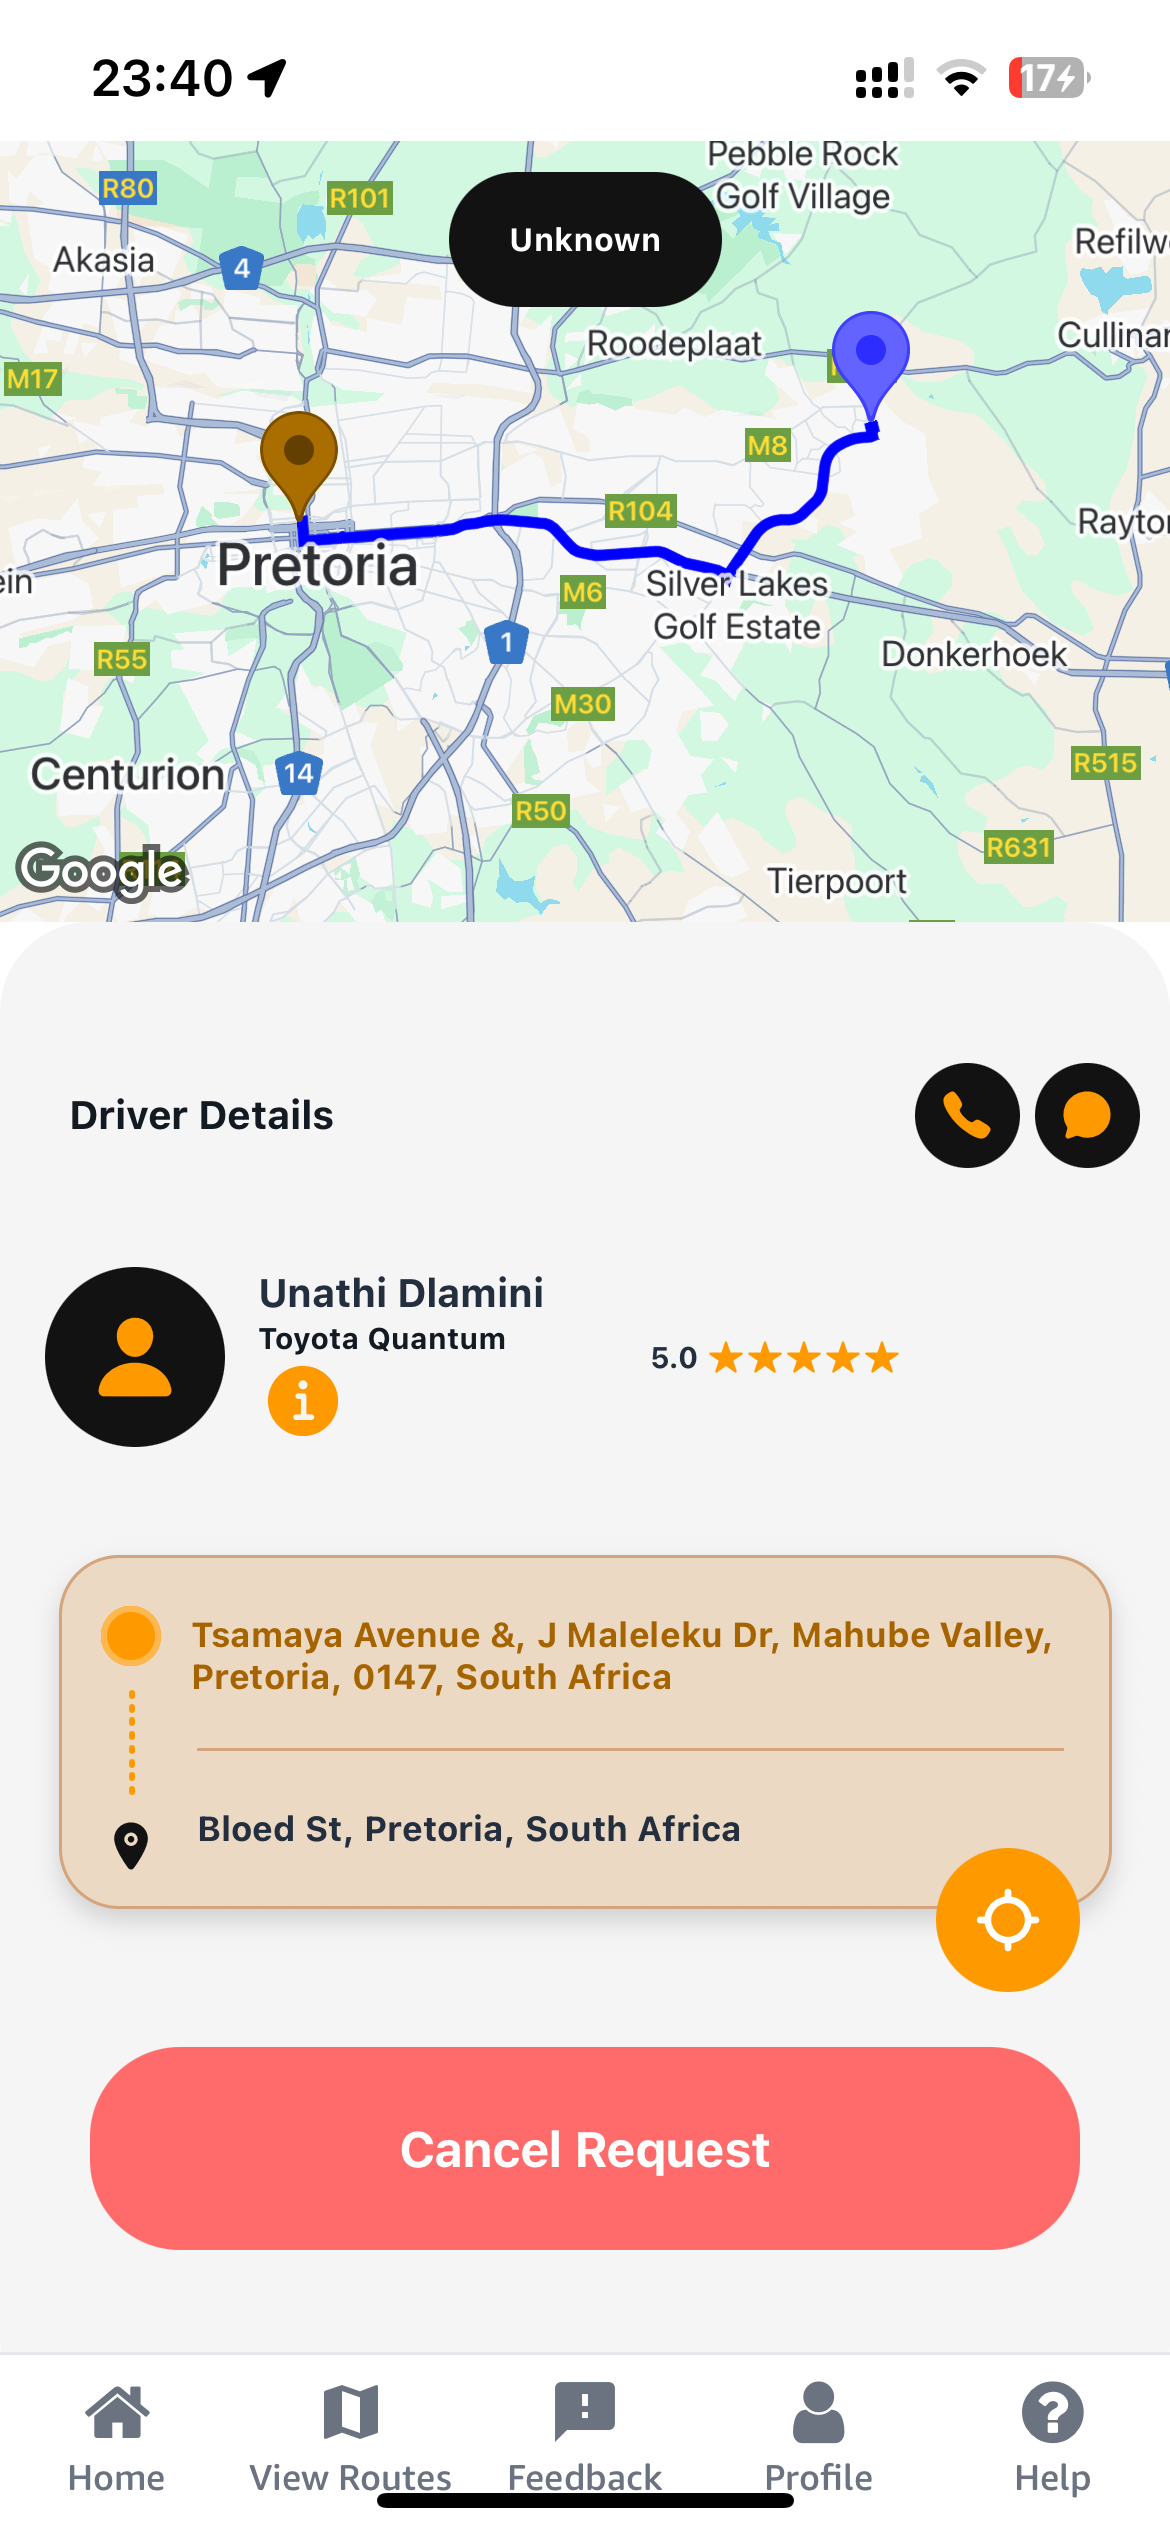
\includegraphics[width=0.4\textwidth]{cancel_request.png}
  \caption{Cancel Request}
\end{figure}

\begin{figure}[H]
  \centering
  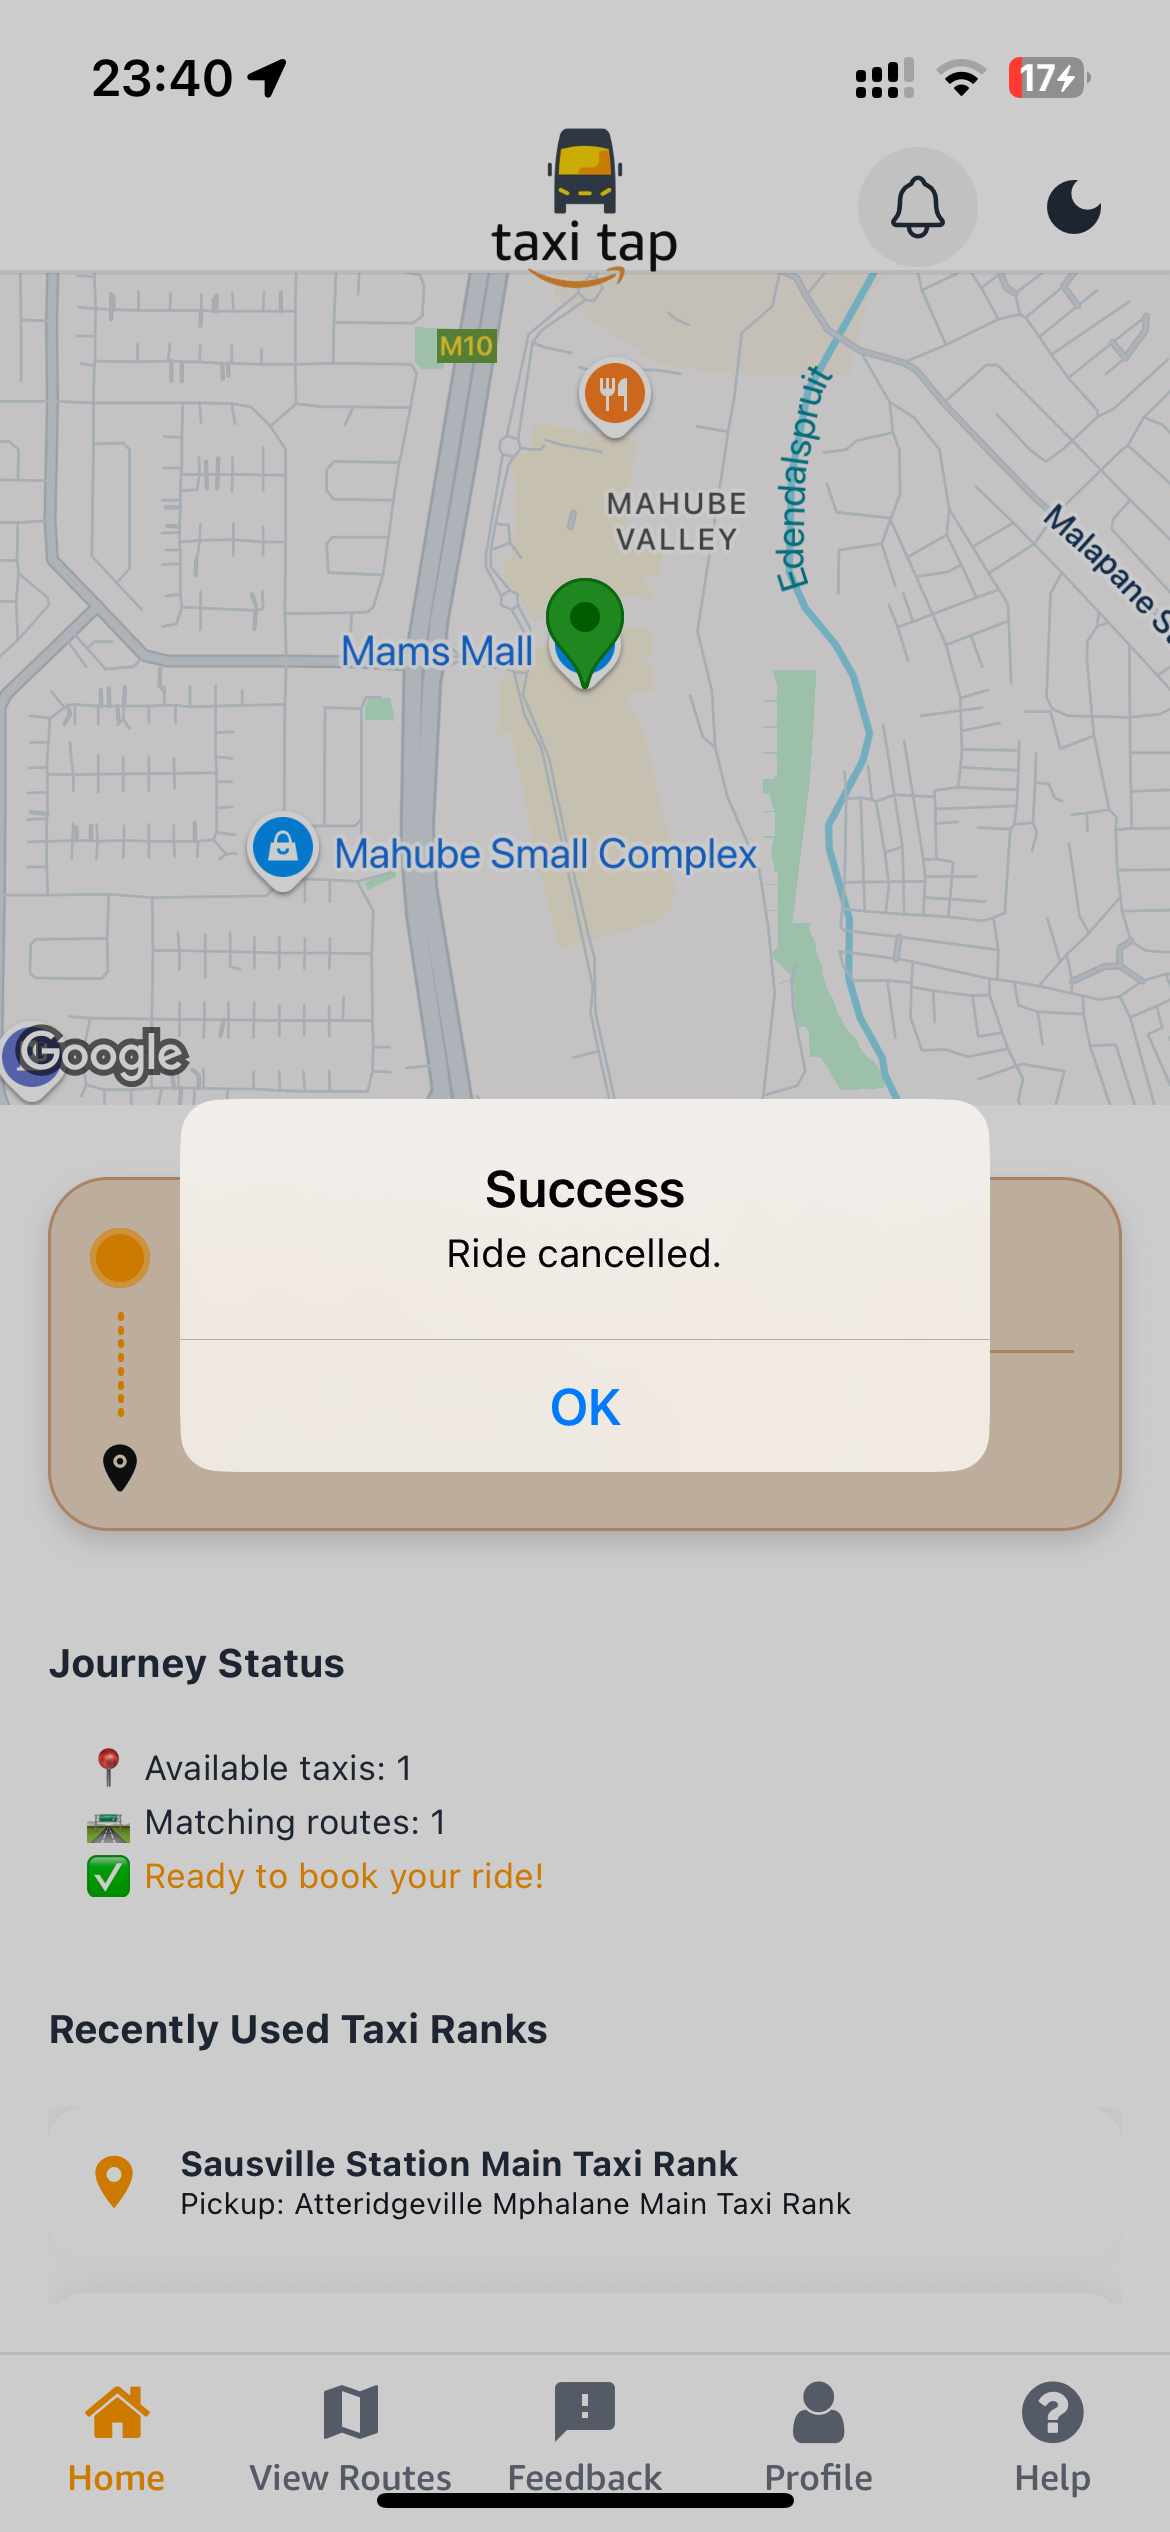
\includegraphics[width=0.4\textwidth]{ride_cancelled.png}
  \caption{Ride Cancellation}
\end{figure}

\section{Driver Interface}

\subsection{Overview}
The Driver interface allows registered drivers to:
\begin{itemize}
    \item Receive ride requests from passengers
    \item Accept or decline requests
    \item Navigate to pickup and drop-off locations
    \item Manage their availability status and seat capacity
    \item Track earnings and ride history
    \item View detailed ride and payment statistics
\end{itemize}

\begin{figure}[H]
  \centering
  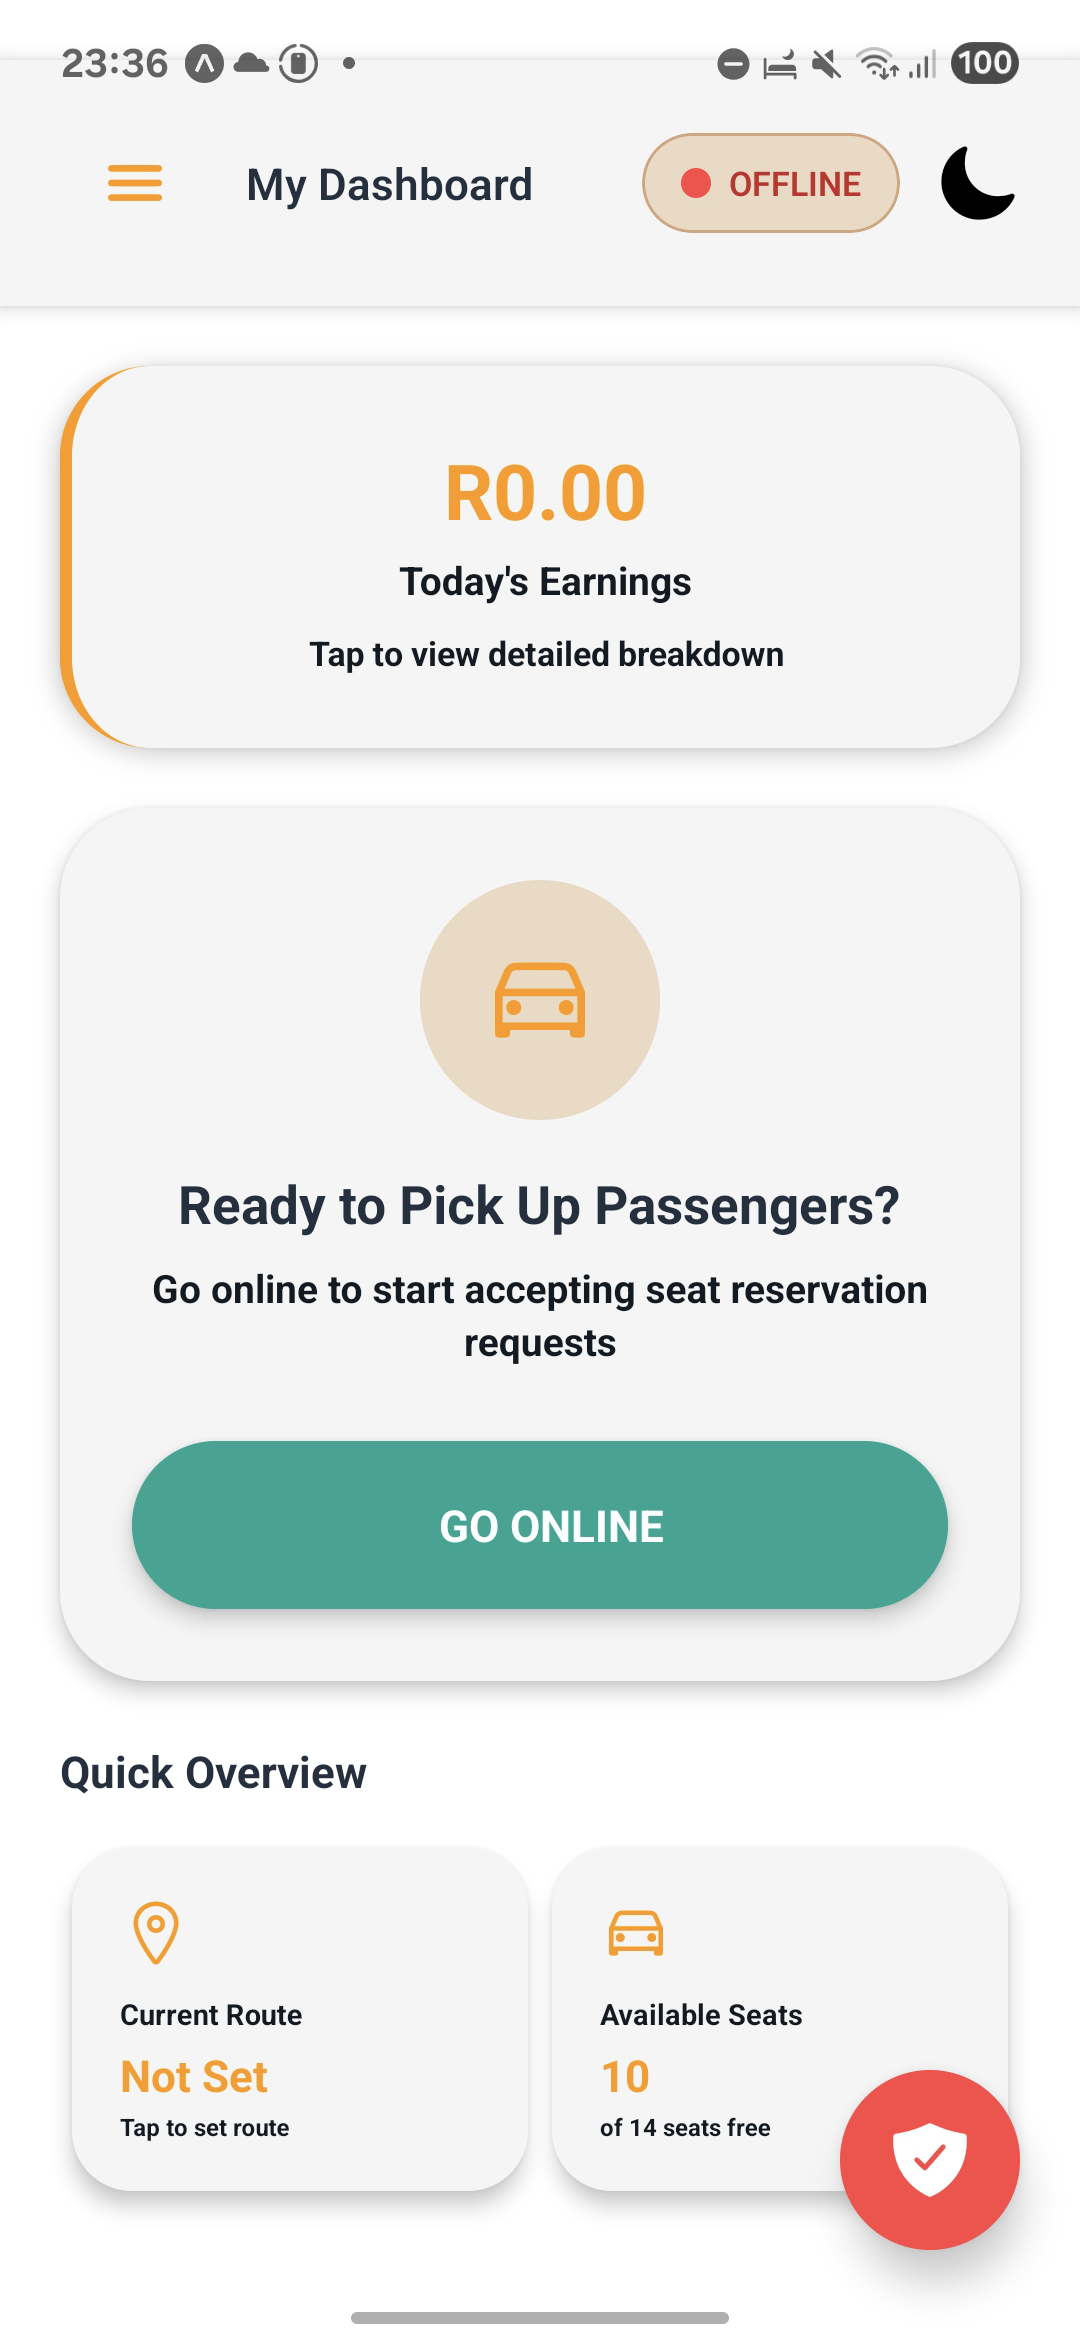
\includegraphics[width=0.4\textwidth]{driver_interface.png}
  \caption{Driver Main Interface}
\end{figure}

\begin{figure}[H]
  \centering
  \includegraphics[width=0.4\textwidth]{driver_interface_2.png}
  \caption{Driver Main Interface}
\end{figure}

\subsection{Managing Availability and Capacity}

\subsubsection{Driver Online Interface}
When online, drivers can:
\begin{itemize}
    \item Manually increase and decrease available seats
    \item View current capacity status
    \item Toggle availability on/off
    \item See incoming ride requests
\end{itemize}

\begin{figure}[H]
  \centering
  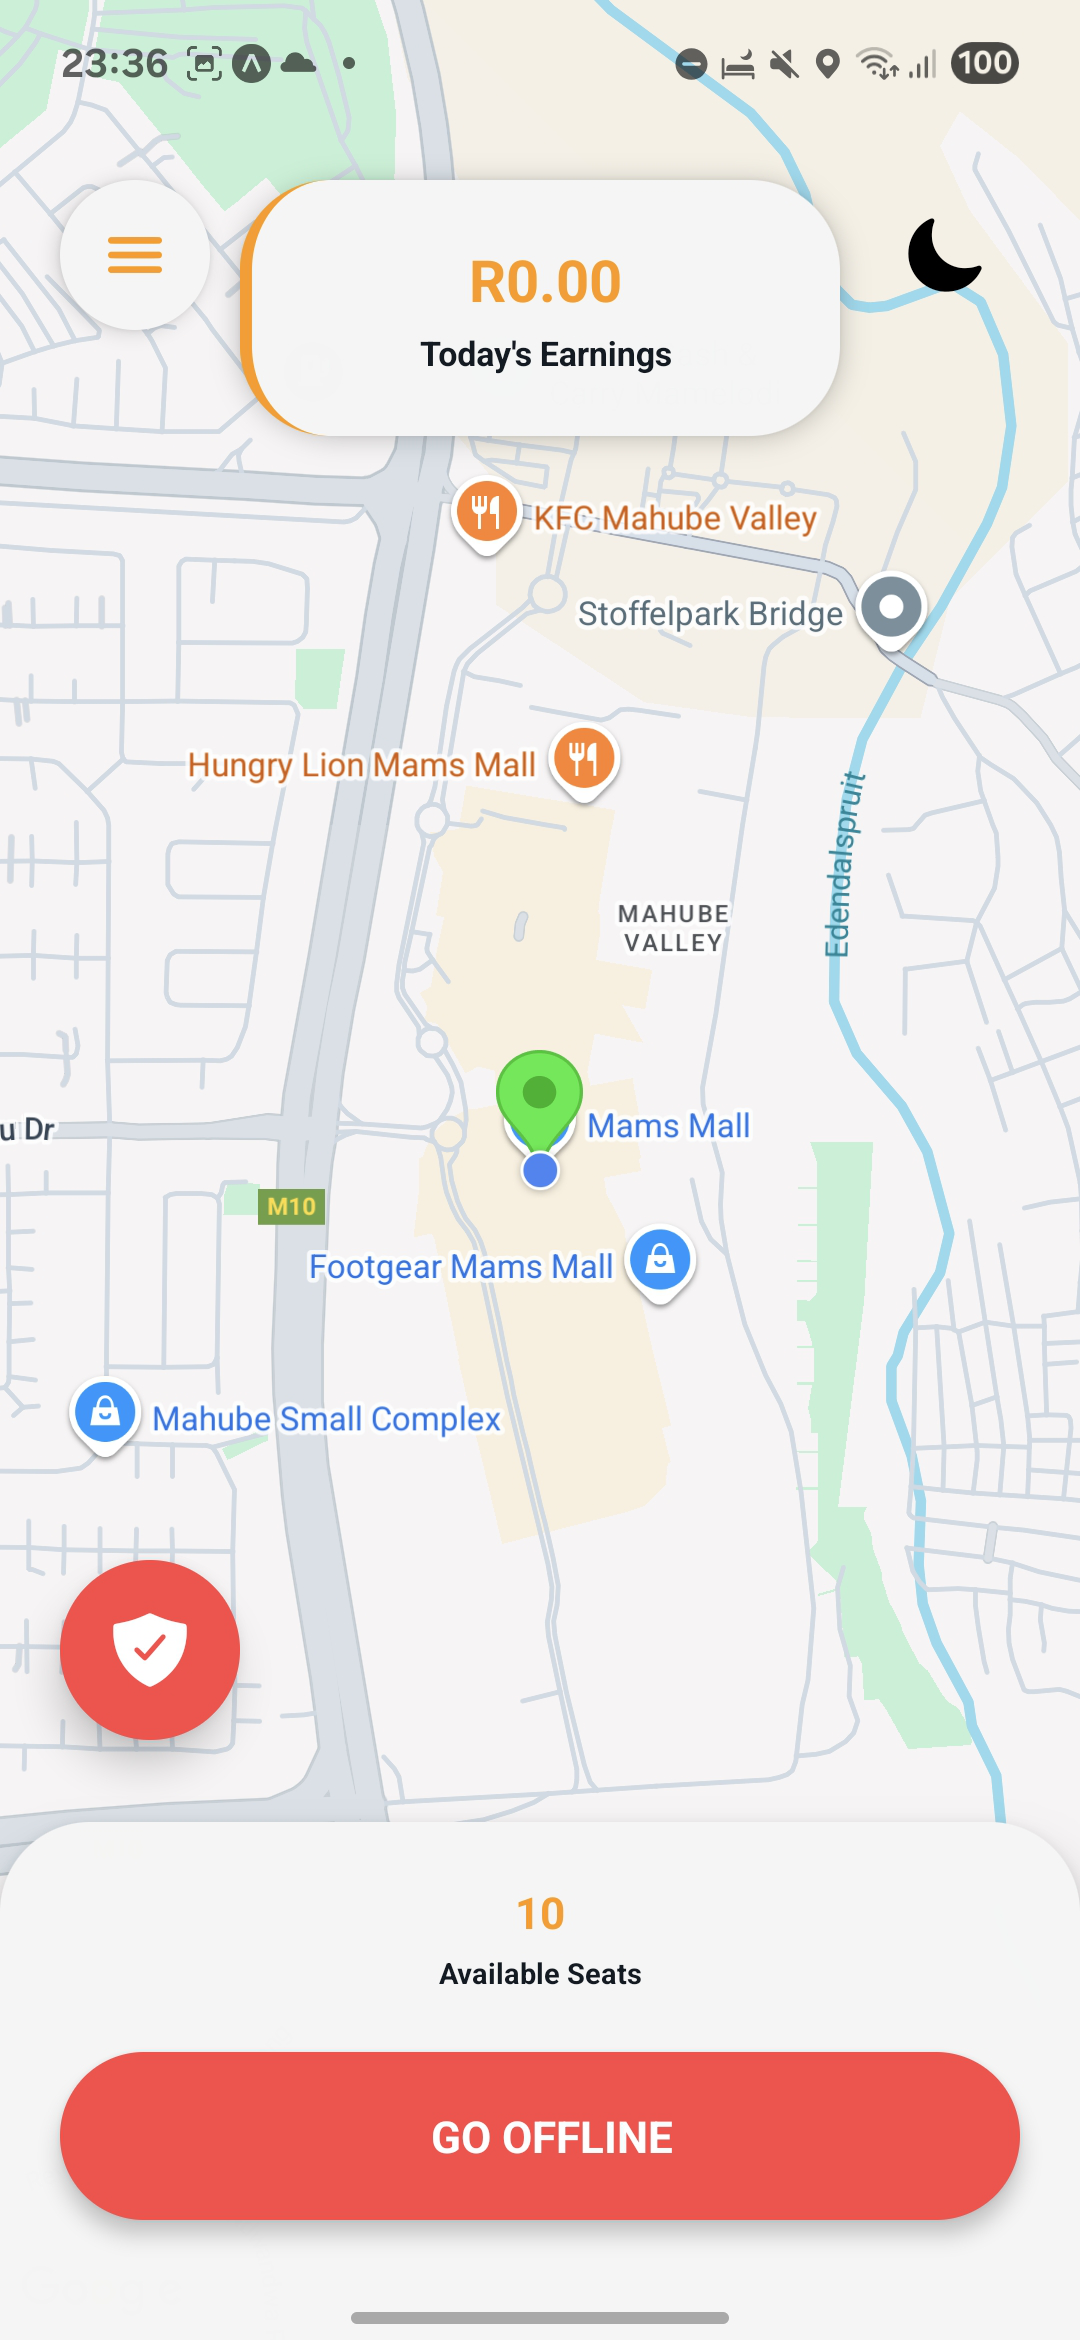
\includegraphics[width=0.4\textwidth]{driver_online.png}
  \caption{Driver Online Interface}
\end{figure}


\subsection{Managing Ride Requests}
\subsubsection{Receiving Requests}
When a passenger requests a ride:
\begin{itemize}
    \item You'll receive a notification with passenger details
    \item The request will show pickup and drop-off locations
    \item You can see the estimated fare and duration
    \item You have the option to accept or decline
\end{itemize}

\subsubsection{Accepting Rides}
To accept a ride request:
\begin{itemize}
    \item Review the trip details
    \item Tap "Accept Ride" if you want to take the request
    \item Navigate to the passenger's pickup location
    \item Provide PIN to passenger for secure boarding confirmation
\end{itemize}

\begin{figure}[H]
  \centering
  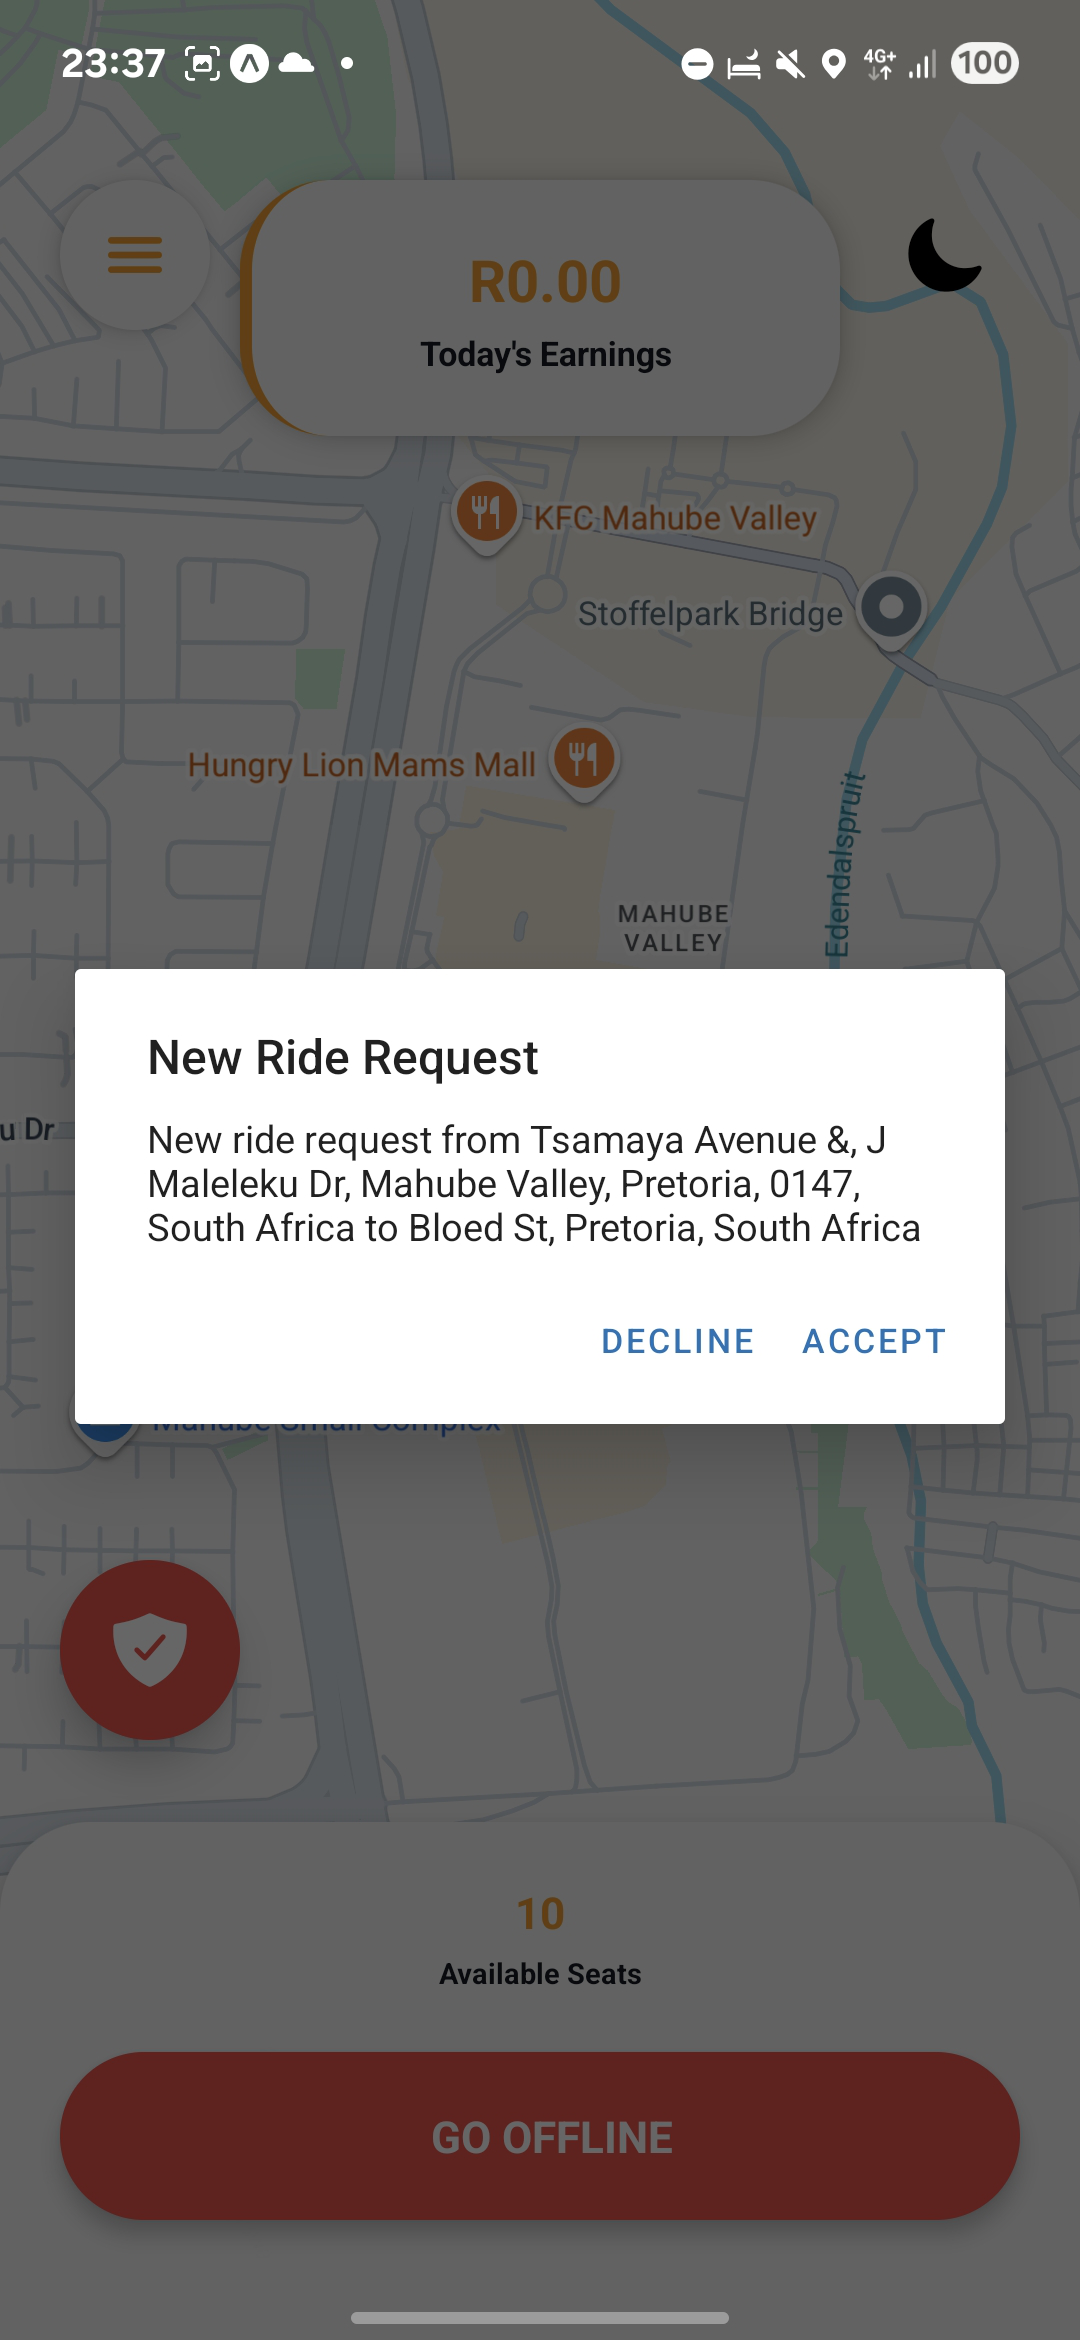
\includegraphics[width=0.4\textwidth]{accept_ride.png}
  \caption{Accept Ride Interface}
\end{figure}

\subsection{Earnings and Statistics}

\subsubsection{Weekly Earnings}
Drivers can view their earnings through a dedicated Earnings page:
\begin{itemize}
    \item Weekly earnings breakdown
    \item Total rides completed
    \item Average fare per ride
    \item Payment status overview
\end{itemize}

\begin{figure}[H]
  \centering
  \includegraphics[width=0.4\textwidth]{weekly_earnings.png}
  \caption{Weekly Earnings Page}
\end{figure}

\subsubsection{Ride and Payment Statistics}
The statistics section provides comprehensive ride management:
\begin{itemize}
    \item Active rides currently in progress
    \item Waiting payment rides (completed but payment pending)
    \item Unpaid rides that require follow-up
    \item Historical ride data and trends
\end{itemize}

\begin{figure}[H]
  \centering
  \includegraphics[width=0.4\textwidth]{ride_payment_stats.png}
  \caption{Ride and Payment Statistics Overview}
\end{figure}

\subsubsection{Active Rides}
View and manage rides currently in progress:
\begin{itemize}
    \item Passenger details and destinations
    \item Current ride status and location
    \item Estimated completion times
    \item Direct communication options
\end{itemize}

\begin{figure}[H]
  \centering
  \includegraphics[width=0.4\textwidth]{active_rides.png}
  \caption{Active Rides Dashboard}
\end{figure}

\subsubsection{Waiting Payment Rides}
Track completed rides awaiting payment:
\begin{itemize}
    \item Recently completed trips
    \item Payment processing status
    \item Passenger contact information for follow-up
    \item Expected payment timeline
\end{itemize}

\begin{figure}[H]
  \centering
  \includegraphics[width=0.4\textwidth]{waiting_payments.png}
  \caption{Waiting Payment Rides}
\end{figure}

\subsubsection{Unpaid Rides}
Manage rides that remain unpaid:
\begin{itemize}
    \item Overdue payment notifications
    \item Passenger contact details
    \item Options for payment follow-up
    \item Dispute resolution tools
\end{itemize}

\begin{figure}[H]
  \centering
  \includegraphics[width=0.4\textwidth]{unpaid_rides.png}
  \caption{Unpaid Rides Management}
\end{figure}

\section{Additional Features}

\subsection{Navigation Features}
\begin{itemize}
    \item View Routes: Access detailed route information
    \item Real-time GPS tracking
    \item Turn-by-turn navigation
    \item Alternative routes
\end{itemize}

\subsection{Support and Feedback}
\begin{itemize}
    \item Feedback: Submit feedback about your experience
    \item Help: Access user guides and FAQs
    \item Profile: Manage your account settings
\end{itemize}

\subsection{Recently Used Taxi Ranks}
The app keeps track of frequently used taxi ranks for quick access:
\begin{itemize}
    \item Sausville Station Main Taxi Rank
    \item Atteridgeville Mphalane Main Taxi Rank
    \item Other commonly used pickup points
\end{itemize}

\section{Troubleshooting}

\subsection{Common Issues}
\subsubsection{No Available Taxis}
If no taxis are available:
\begin{itemize}
    \item Check if your location is within the service area
    \item Try requesting again after a few minutes
    \item Consider alternative pickup locations nearby
\end{itemize}

\subsubsection{Connection Issues}
If you experience connectivity problems:
\begin{itemize}
    \item Ensure you have a stable internet connection
    \item Check your GPS settings are enabled
    \item Restart the app if necessary
\end{itemize}

\section{Safety Guidelines}

\subsection{For Passengers}
\begin{itemize}
    \item Verify driver and vehicle details before boarding
    \item Confirm PIN with driver for secure ride start
    \item Share your trip details with trusted contacts
    \item Use in-app emergency features when needed
    \item Rate your experience to help maintain service quality
\end{itemize}

\subsection{For Drivers}
\begin{itemize}
    \item Maintain vehicle safety standards
    \item Verify passenger identity and provide PIN before pickup
    \item Follow designated routes and traffic laws
    \item Report any safety concerns immediately
    \item Keep accurate records of payments and ride status
\end{itemize}

\section{Contact Information}

For technical support, feedback, or general inquiries:
\begin{itemize}
    \item Email: \href{mailto:gititdone.2025@gmail.com}{gititdone.2025@gmail.com}\\
    \item Website: \url{http://www.gititdone2025.site}
\end{itemize}

Developed by Git It Done Team

\end{document}